% This must be in the first 5 lines to tell arXiv to use pdfLaTeX, which is strongly recommended.
% \pdfoutput=1
% In particular, the hyperref package requires pdfLaTeX in order to break URLs across lines.

\documentclass[11pt]{article}

% Change "review" to "final" to generate the final (sometimes called camera-ready) version.
% Change to "preprint" to generate a non-anonymous version with page numbers.
% \usepackage[review]{acl}
\usepackage[final]{acl}

% Standard package includes
\usepackage{times}
\usepackage{latexsym}

% For proper rendering and hyphenation of words containing Latin characters (including in bib files)
% \usepackage[T1]{fontenc}
% For Vietnamese characters
% \usepackage[T5]{fontenc}
% See https://www.latex-project.org/help/documentation/encguide.pdf for other character sets

% This assumes your files are encoded as UTF8
% \usepackage[utf8]{inputenc}

% This is not strictly necessary, and may be commented out,
% but it will improve the layout of the manuscript,
% and will typically save some space.
\usepackage{microtype}

% This is also not strictly necessary, and may be commented out.
% However, it will improve the aesthetics of text in
% the typewriter font.
\usepackage{inconsolata}

%Including images in your LaTeX document requires adding
%additional package(s)
\usepackage{graphicx}
\usepackage[UTF8,fontset=fandol]{ctex}

% If the title and author information does not fit in the area allocated, uncomment the following
%
%\setlength\titlebox{<dim>}
%
% and set <dim> to something 5cm or larger.

% My packages are here
\usepackage{algorithmic}
\usepackage{algorithm}
\usepackage{amssymb}
\usepackage{amsmath}
\usepackage{xcolor}
% \usepackage{algpseudocode}
\usepackage{tikz}
\usetikzlibrary{calc}
\usetikzlibrary{matrix}
\usetikzlibrary{shapes.arrows}
\usetikzlibrary{decorations.pathreplacing,calligraphy}
\usetikzlibrary{patterns}
\usepackage{pgfplots}
\usepackage{pgfplotstable}
\usepackage{subcaption}
\usepackage{multirow}
\usepackage{enumitem}
\definecolor{darkteal}{HTML}{2E5F7F}

\let\oldequation\equation
\let\oldendequation\endequation
\renewenvironment{equation}{\small\oldequation}{\oldendequation}

\newcommand{\paperName}{KVPR}

\title{\paperName：基于 I/O 感知 KV 缓存部分重计算的高效 LLM 推理}

% Author information can be set in various styles:
% For several authors from the same institution:
% \author{Author 1 \and ... \and Author n \\
%         Address line \\ ... \\ Address line}
% if the names do not fit well on one line use
%         Author 1 \\ {\bf Author 2} \\ ... \\ {\bf Author n} \\
% For authors from different institutions:
% \author{Author 1 \\ Address line \\  ... \\ Address line
%         \And  ... \And
%         Author n \\ Address line \\ ... \\ Address line}
% To start a separate ``row'' of authors use \AND, as in
% \author{Author 1 \\ Address line \\  ... \\ Address line
%         \AND
%         Author 2 \\ Address line \\ ... \\ Address line \And
%         Author 3 \\ Address line \\ ... \\ Address line}

% \author{First Author \\
%   Affiliation / Address line 1 \\
%   Affiliation / Address line 2 \\
%   Affiliation / Address line 3 \\
%   \texttt{email@domain} \\\And
%   Second Author \\
%   Affiliation / Address line 1 \\
%   Affiliation / Address line 2 \\
%   Affiliation / Address line 3 \\
%   \texttt{email@domain} \\}

\author{%
  Chaoyi Jiang$^{*}$, Lei Gao\thanks{These authors contributed equally.}, Hossein Entezari Zarch, Murali Annavarm\\
  University of Southern California\\
  \texttt{\{chaoyij, leig, entezari, annavara\}@usc.edu}\\
}

\renewcommand{\contentsname}{目录}
\renewcommand{\tablename}{表}
\renewcommand{\figurename}{图}
\renewcommand{\abstractname}{摘要}
\begin{document}

\maketitle

\begin{abstract}
大语言模型（LLM）推理计算开销很高。为降低自回归解码成本，系统通常使用 Key-Value（KV）缓存保存中间激活，从而显著降低 token 生成的计算开销。然而，KV 缓存所需内存会快速增长，常常超过 GPU 显存容量。一种成本更低的替代方案是将 KV 缓存卸载到 CPU 内存，以缓解 GPU 显存压力，但这又把瓶颈转移到 CPU 与 GPU 之间 PCIe 连接的有限带宽上。现有方法尝试通过重叠 GPU 计算与 I/O，或采用 CPU-GPU 异构执行来缓解这些问题，但它们会受到过量数据移动和 CPU 能力依赖的限制。随着 KV 缓存增大和/或 GPU 计算能力增强，完全隐藏 PCIe 通信延迟会变得越来越困难。本文提出 KVPR，一种高效的 I/O 感知 LLM 推理方法：CPU 先传输一部分激活值，GPU 基于这些激活值开始重计算 KV 缓存；在 GPU 重计算部分 KV 缓存的同时，CPU 并发传输剩余 KV 缓存。该方法通过重叠 GPU 重计算与 KV 缓存传输，最小化 GPU 空闲时间并最大化推理性能。KVPR 通过集成 profiler、scheduler 和 runtime 实现全自动化：profiler 利用输入特征和系统硬件信息，scheduler 优化计算与通信工作负载划分，runtime 高效执行生成的执行计划。实验结果表明，相比当前最先进方法，KVPR 在解码阶段最高降低 35.8\% 延迟，并提升 46.2\% 吞吐量。代码已开源：\url{https://github.com/chaoyij/KVPR}。
\end{abstract}


\section{引言}
近年来，大型语言模型 (LLM) 取得了显著进展，展示了它们为机器翻译等多种应用提供支持的能力 \cite{zhu2024multilingual}, 总结 \cite{openai2024gpt4}、创意内容生成 \cite{geminiteam2024gemini}，以及个性化推荐 \cite{geng2022p5}。实时应用程序，包括对话代理和实时翻译 \cite{li2023camel}，依靠低延迟来提供无缝的用户交互，而大规模部署则需要高吞吐量来支持并发用户并高效处理大量数据 \cite{kwon2023vllm}。

键值 (KV) 缓存对于 LLM 的自回归解码至关重要，因为它存储注意力机制中早期步骤的中间键和值激活。通过消除为每个生成的令牌重计算这些激活的需要，这降低了生成每个令牌从二次到线性的计算复杂性。然而，这是有代价的：KV 缓存的大小随着批量大小、序列长度和模型大小线性增长，导致大量的内存需求 \cite{wan2024efficient}.

GPU 内存虽然针对计算单元的高带宽访问进行了优化，但本质上是有限的，并且通常不足以处理庞大且不断增长的 KV 缓存。解决这一限制的一种经济高效的方法是将 KV 缓存卸载到更便宜且充足的 CPU 内存，并且可以进一步卸载到硬盘和网络存储 \cite{liu2024cachegen}。虽然卸载减少了 GPU 内存压力，但它引入了一个新的瓶颈：缓慢的 PCIe 总线成为将 KV 缓存从 CPU 转移到 GPU 进行计算时的限制因素。由于PCIe传输时间较长，导致整体解码延迟增加，令牌生成吞吐量下降，阻碍了系统的整体推理效率 \cite{zhao2024hetegen}.

\begin{figure}
    \centering
    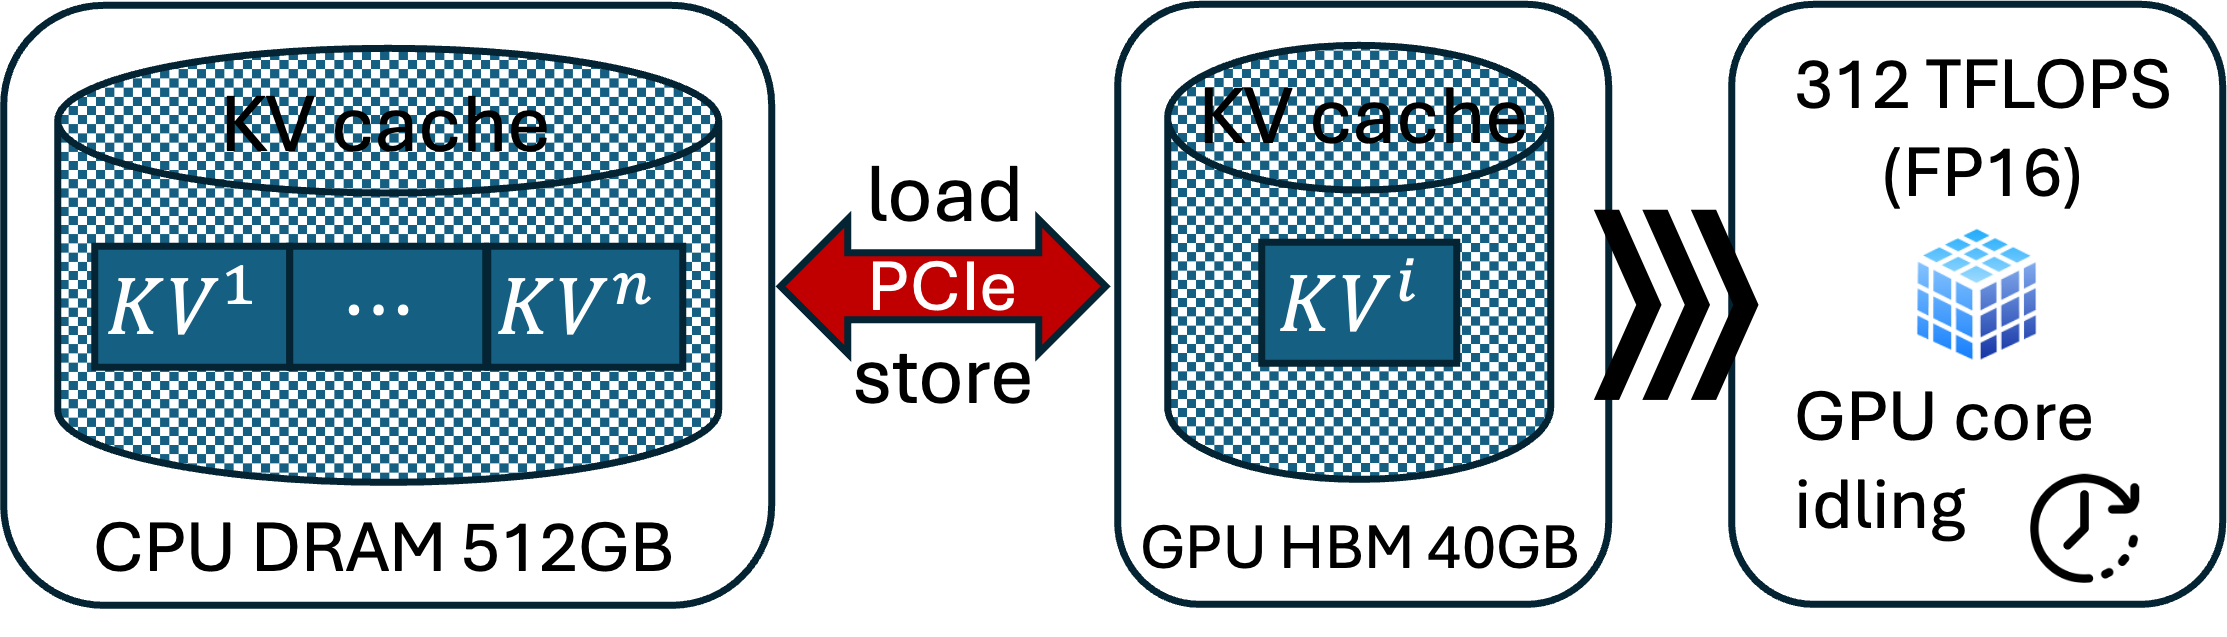
\includegraphics[width=1\columnwidth]{assets/intro.png}
    \caption{配备 A100 GPU 的 LLM 推理系统。}
    \label{fig:intro}
\end{figure}


\begin{table}[h]
\centering
\resizebox{\columnwidth}{!}{%
\begin{tabular}{lcccc}
\hline
\textbf{Model} & \multicolumn{1}{l}{\textbf{Hidden Dim}} & \textbf{\begin{tabular}[c]{@{}c@{}}KV Cache \\ (MB)\end{tabular}} & \textbf{\begin{tabular}[c]{@{}c@{}}PCIe Latency \\ (ms)\end{tabular}} & \textbf{\begin{tabular}[c]{@{}c@{}}Comp. Latency\\ (ms)\end{tabular}} \\ \hline
OPT-6.7B & 4,096 & 512 & 15.6 & 0.3509 \\
OPT-13B & 5,120 & 640 & 19.5 & 0.4388 \\
OPT-30B & 7,168 & 896 & 27.3 & 0.6143 \\ \hline
\end{tabular}%
}
\caption{图 \ref{fig:intro} 所示系统中，不同 KV 缓存大小对应的 PCIe 延迟和计算延迟。}
\label{tab:slow-pcie}
\end{table}

% 2*5120*1024*32*2*40/1024**3 = 25GB
为了评估通信开销的影响，我们建立了如图 \ref{fig:intro} 所示的 LLM 推理服务系统，使用 NVIDIA A100 GPU。CPU DRAM 和 GPU HBM 之间的数据传输通过 PCIe 4.0 x16 完成，带宽为 32 GB/s。表 \ref{tab:slow-pcie} 展示了不同模型的隐藏维度、KV 缓存大小、PCIe 传输时间和 GPU 计算延迟。请注意，端到端解码延迟还包含前馈层等其他组件；为清楚起见，这些组件未在表中列出。我们使用 FP16 精度、批量大小 32、序列长度 1024。结果表明，PCIe 延迟比 KV 缓存重计算延迟高一个数量级以上。因此，在 KV 缓存存储于 CPU DRAM 的系统中，较长的数据传输时间会造成 GPU 空闲，损害推理效率。 

为了缓解 PCIe 延迟和带宽问题，FlexGen \cite{sheng2023flexgen} 和 PipeSwitch \cite{bai2020pipeswitch} 尝试将当前层的 GPU 计算与下一层的 KV 缓存加载重叠。然而，这种重叠的有效性受到耗时最长任务的限制。在大多数系统中，PCIe 传输时间超过 GPU 计算延迟，尤其是在批量和上下文较大的情况下。因此，完全用 GPU 计算隐藏 PCIe 传输时间并不现实。 % this approach is useful in a setting where the data transfer time and GPU computation time are similar, which is generally not the case with large batch and context sizes. 
FastDecode \cite{he2024fastdecode} 建议直接在 CPU 上计算注意力分数，与 GPU 相比，CPU 可以更快地访问 KV 缓存。同样，HeteGen \cite{zhao2024hetegen}, TwinPilots \cite{yu2024twinpilots}， 和 \citeauthor{park2024improving} 采用 CPU-GPU 异构执行，通过在 CPU 上执行计算来隐藏数据传输开销。然而，正如我们稍后的结果所证明的，这种方法给 CPU 带来了负担，无法满足连接到 CPU 主机的多个 GPU 的 KV 缓存计算需求，从而限制了可扩展性。   


本文提出 \paperName，一种面向高效 LLM 推理的新方法，用于平衡 GPU 计算与 PCIe 带宽之间的取舍。CPU 不再把整个 KV 缓存从 CPU 传输到 GPU 后再计算注意力分数，而是先将更小的部分激活集传输到 GPU，这些激活可用于生成一部分 KV 缓存。随后 GPU 根据输入激活重计算部分 KV 缓存；与此同时，CPU 通过 PCIe 传输剩余 KV 缓存。{\paperName} 在不引入近似的前提下计算精确注意力分数，并最大限度减少 GPU 空闲时间，从而改善整体延迟和吞吐量。

{\paperName} 通过确定需要重计算的激活比例，使 PCIe 传输时间与 GPU 重计算时间实现\textit{近乎完美}的重叠。{\paperName} 可自动确定重计算与通信之间的切分：profiler 收集系统硬件信息，scheduler 将问题表述为线性规划以确定最优切分点，runtime 管理两个设备上的内存分配并协调数据传输。实验结果表明，根据不同工作负载，{\paperName} 可显著降低推理延迟或提高吞吐量。总之，我们的贡献如下：

\begin{itemize}[topsep=0pt, partopsep=0pt, parsep=0pt, itemsep=2pt]
    \item 我们提出了一种高效的 CPU-GPU I/O 感知 LLM 推理方法，该方法利用 KV 缓存部分重计算和异步 KV 缓存传输（重叠计算和通信）来解决从 CPU 内存加载大型 KV 缓存的系统瓶颈。
    \item 我们开发了一个基于线性整数规划的框架，可实现最佳的计算通信分配。
    \item 实验结果表明，{\paperName} 相比当前最先进方法最高可降低 35.8\% 延迟，并提升 46.2\% 吞吐量。
\end{itemize}



\section{背景}

\textbf{LLM 推理过程。}
仅解码器 LLM 的推理过程采用自回归方法，顺序生成 token。它由两个阶段组成： \textbf{预填充阶段} 和 \textbf{解码阶段}。 
在预填充阶段，第 $i$ 个解码器层的输入表示为 $ X^i \in \mathbb{R}^{b \times s \times h} $，其中 $i \in \{1,\ldots,n\} $，$ b $ 是批量大小，$ s $ 是提示长度，$ h $ 是输入嵌入维度。多头注意力（MHA）块通过对 $ X^i $ 做线性投影来计算查询（$ Q $）、键（$ K $）和值（$ V $）：


\begin{equation}
Q^i = X^i \cdot W^i_Q, \quad K^i = X^i \cdot W^i_K, \quad V^i = X^i \cdot W^i_V,
\label{eq:mha_projection}
\end{equation}
其中 $ W^i_Q, W^i_K, W^i_V \in \mathbb{R}^{h \times h} $ 是投影矩阵。生成的 $K^i$ 和 $V^i$ 存储在 KV 缓存中。

\noindent MHA 中的自注意力分数计算如下：

\begin{equation}
Z^i = \text{softmax}\left(\frac{Q^i (K^i)^T}{\sqrt{d_{\text{head}}}}\right) \cdot V^i,
\label{eq:attention}
\end{equation}
其中 $ d_{\text{head}} $ 表示每个注意力头的维度。 
最后，将注意力分数与线性投影一起应用以产生 MHA 块的输出：

\begin{equation}
O^i = Z^i \cdot W^i_O,
\label{eq:mha_output}
\end{equation}
其中 $ W^i_O \in \mathbb{R}^{h \times h} $ 是投影矩阵。

MHA 块之后是前馈网络 (FFN)，它由两个完全连接的层组成，在它们之间应用了非线性激活函数。 
它处理注意力输出 $ O^i $ 生成下一个解码器层的输入，如下所示：

\begin{equation}
X^{i+1} = \sigma(O^i \cdot W^i_1) \cdot W^i_2,
\label{eq:ffn}
\end{equation}
其中 $ W^i_1 \in \mathbb{R}^{h \times d_{\text{FFN}}} $ 和 $ W^i_2 \in \mathbb{R}^{d_{\text{FFN}} \times h} $ 是两个线性层的权重矩阵，$ \sigma(\cdot) $ 表示激活函数。

在解码阶段，第 $i$ 个解码器层接收单个 token $ x^i \in \mathbb{R}^{b \times 1 \times h} $。通过将新计算的键值对与已有键值对拼接来更新 KV 缓存：

% \begin{equation}
% K^i = \text{concat}(K^i, x^i \cdot W^i_K), \quad V^i = \text{concat}(V^i, x^i \cdot W^i_V).
% \label{eq:kv_update}
% \end{equation}

\begin{equation}
\begin{aligned}
K^i &= \text{concat}(K^i, x^i \cdot W^i_K), \\
V^i &= \text{concat}(V^i, x^i \cdot W^i_V).
\end{aligned}
\label{eq:kv_update}
\end{equation}

解码阶段中剩余的注意力和前馈计算与预填充阶段中的相同。


\section{方法}
\textbf{LLM 推理调度。} 我们的方法针对具有大型 KV 缓存的 LLM 推理系统，这些缓存存储在 CPU DRAM 上并根据需要提取到 GPU 内存中。由于 LLM 有许多层和许多批次的输入需要处理，因此有不同的调度策略来确定如何跨批次和层执行计算，以优化特定的性能目标，例如最小化延迟或最大化吞吐量。  
逐行排程（如附录所示） \ref{app:schedule}）使用分层执行一次处理一批。在这种情况下，只要可行，模型权重就会保存在 GPU 内存中。如果模型权重也卸载到 CPU，则 KV 缓存和单层的模型权重都会传输到 GPU，针对当前批次进行处理，然后清除。这个过程逐层重复，直到生成令牌。当最大程度地减少延迟是主要目标时，首选此方法，因为批次中的所有提示都经过完全处理，以在继续下一个批次之前生成完整的上下文。

逐列调度（附录 \ref{app:schedule}）通过增加 \emph{有效批量大小} （批次数量乘以批次大小）并行处理更多序列，但代价是更长的延迟。在这种方法中，模型权重被卸载到 CPU 内存以适应大批量。单层的模型权重和 KV 缓存将传输到 GPU 内存并进行第一批处理。当前批次不会移至下一层，而是使用同一层处理后续批次，同时保持权重在 GPU 内存中固定。一旦第一层处理了一组批次，每个批次的处理就会转移到第二层。请注意，有效批量大小受到激活和 KV 缓存的可用存储的限制，因为一旦超过 GPU 内存容量，它们仍必须存储在 CPU 内存或外部存储中。 

我们提出的设计独立于调度策略，无论是逐行还是逐列，旨在将大部分 PCIe 传输时间与 GPU 计算重叠，从而提高整体效率。


\subsection{设计概览}

\begin{figure*}
    \centering
    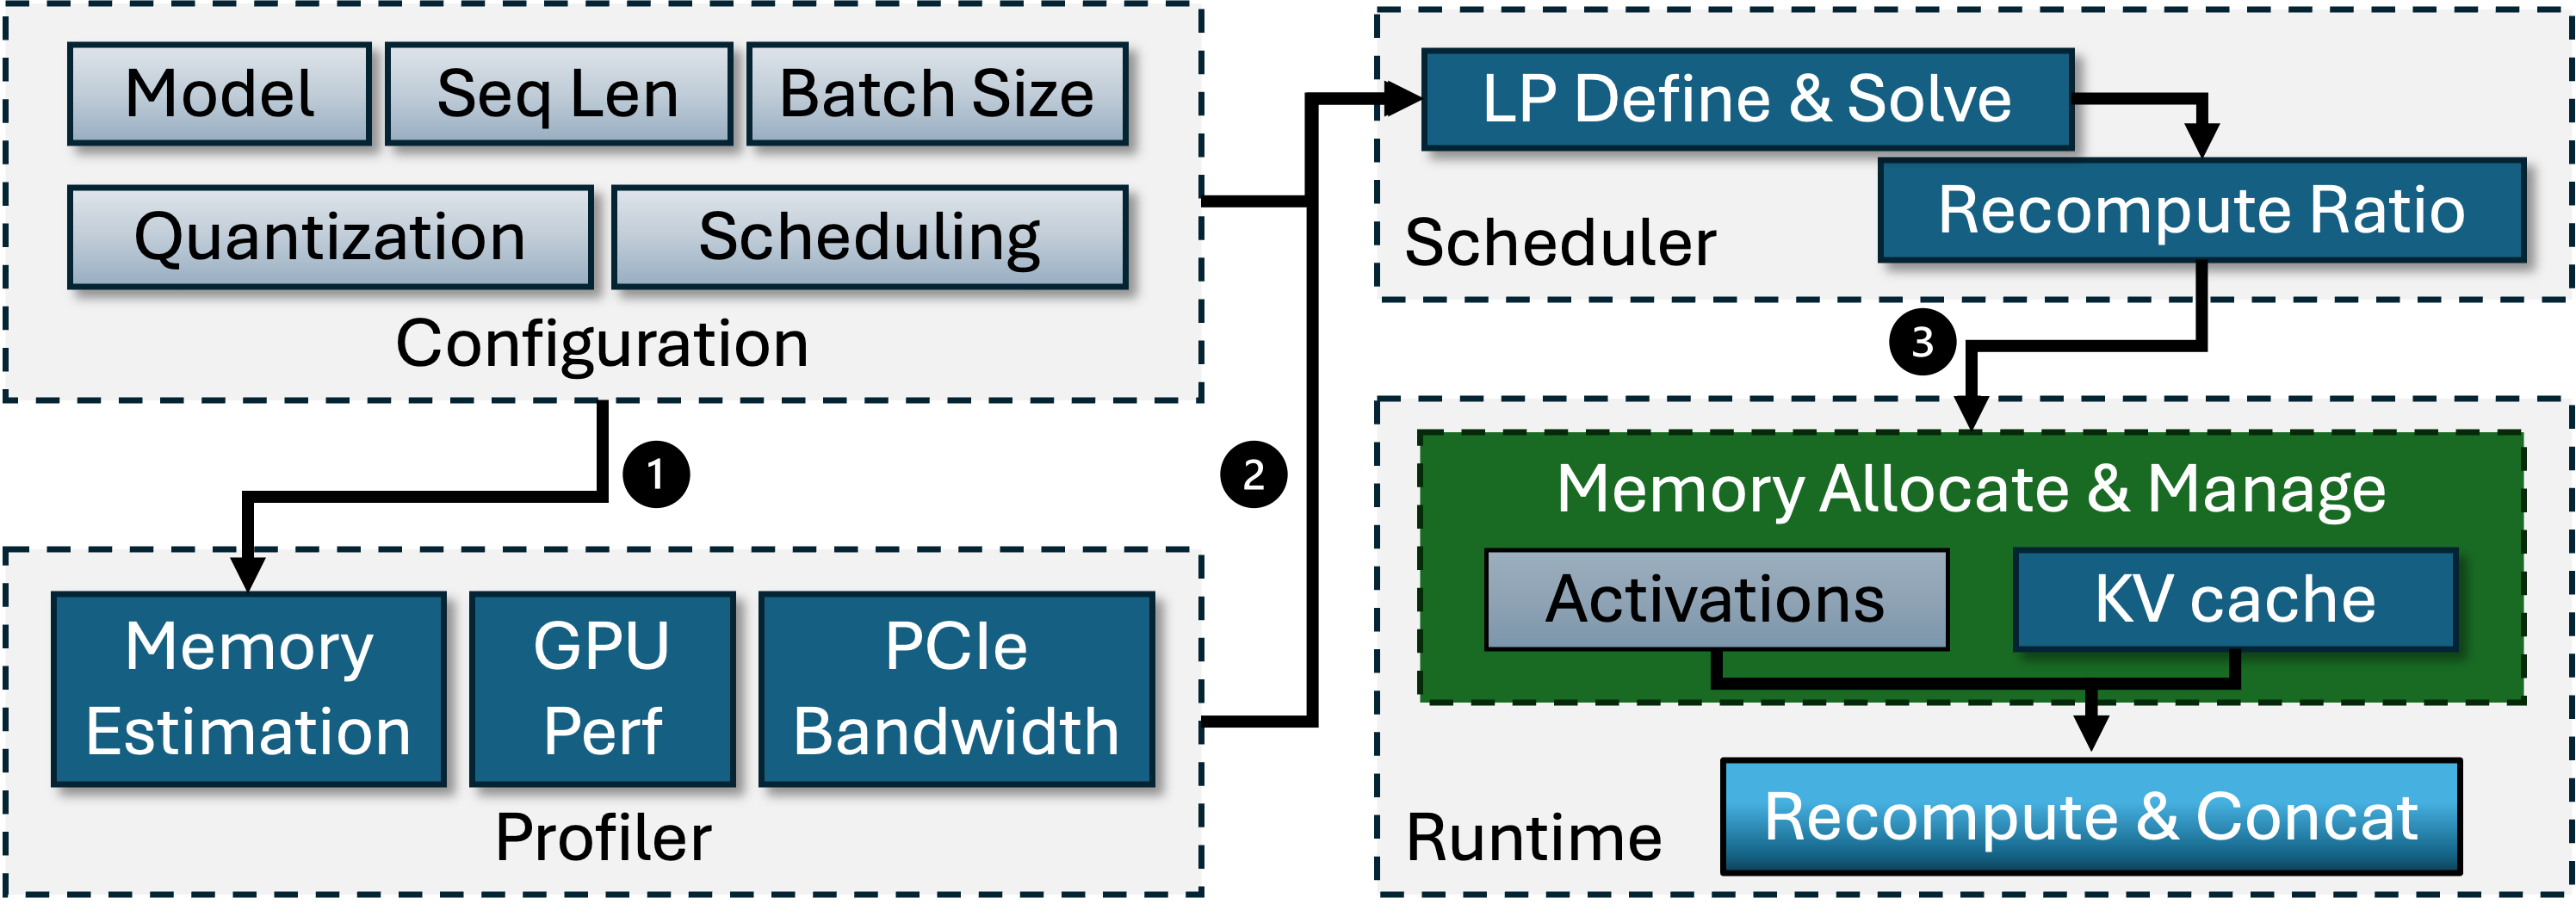
\includegraphics[width=0.7\textwidth]{assets/system.png}
    \caption{{\paperName} 的设计概览。用户配置和 profiler 信息输入 scheduler，scheduler 计算最佳 KV 缓存重计算比例；随后 runtime 重叠数据传输和 GPU 计算以提升推理效率。}
    \label{fig:design-overview}
\end{figure*}

\noindent 为了缓解 PCIe 压力并提高 GPU 计算利用率，我们提出了一种新方法， {\paperName}，重计算 GPU 上的部分 KV 缓存，同时将其余 KV 缓存传输到 GPU。如图 \ref{fig:design-overview}, {\paperName} 包括三个主要模块：分析器、调度器和运行时。 
用户配置包括性能目标（即延迟或吞吐量）、数据参数（例如提示长度、生成长度、批量大小）以及模型信息（例如输入嵌入维度和层数）。 
\textbf{分析器模块}收集系统统计数据，以刻画 PCIe 带宽、GPU 处理速度等硬件特性。例如，分析器模块利用批量大小、模型信息和序列长度来表征 PCIe 带宽。结合这些信息和用户配置，\textbf{调度模块}通过求解线性规划问题来计算最优 KV 缓存重计算切分点，目标是在推理过程中最大化计算与通信的重叠，以及 GPU 和 PCIe 带宽利用率。\textbf{运行时模块}则使用该执行策略处理用户输入，并管理内存分配和数据传输流。 

\subsection{调度器模块}
在本节中，我们将描述如何 {\paperName} 适用于逐行或逐列计划。 

\noindent \textbf{具有 KV 缓存部分重计算的逐行调度。}
如果性能目标是最小化延迟，则调度程序模块将启动逐行执行计划。逐行调度的朴素卸载管道如图所示 \ref{fig:row-by-row}(a)，其中 KV 缓存和模型权重都被卸载到 CPU 内存。所需数据通过 PCIe 异步传输到 GPU 以执行 MHA 和 FFN 块。为了简单起见，图中省略了将新生成的 KV 对存储到 CPU 内存的过程。 
由于 KV 缓存的大小比 MHA 权重更大，因此在异步传输过程中它会较晚到达 GPU。如果模型权重未卸载到 CPU，则管道会略有不同。在这种情况下，只有MHA块会等待KV 缓存数据传输到GPU才开始计算。



\begin{figure}[h]
\centering
\begin{subfigure}[b]{\columnwidth}
    \centering
    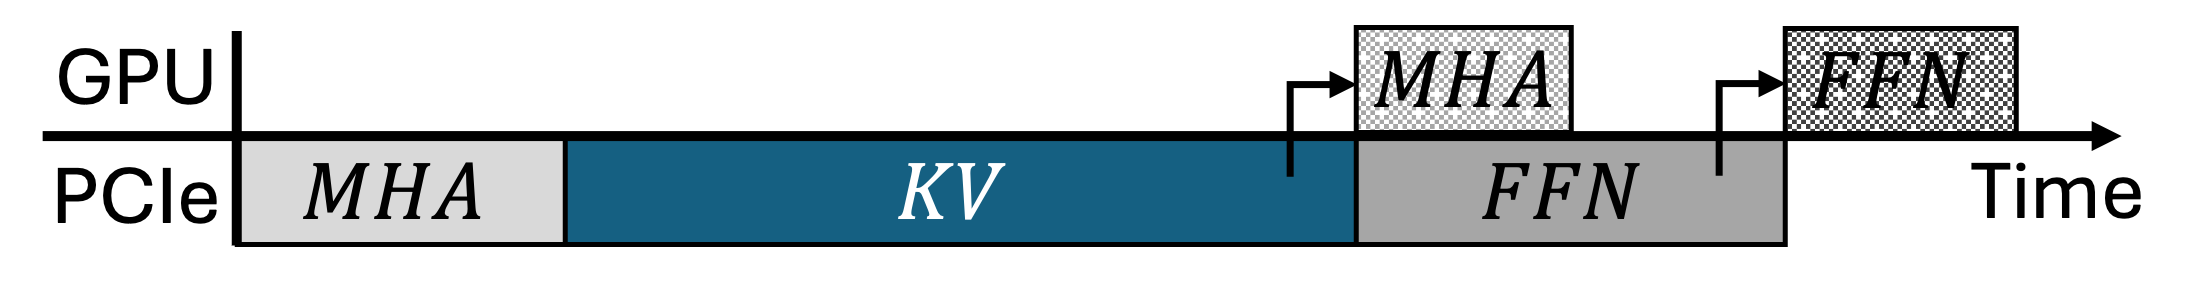
\includegraphics[width=\columnwidth]{assets/3a.png}
    \caption{带异步数据传输的逐行调度朴素卸载管道。GPU 和 PCIe 分别表示 GPU 计算和数据传输，箭头表示数据依赖关系。}
\end{subfigure}

\begin{subfigure}[b]{\columnwidth}
    \centering
    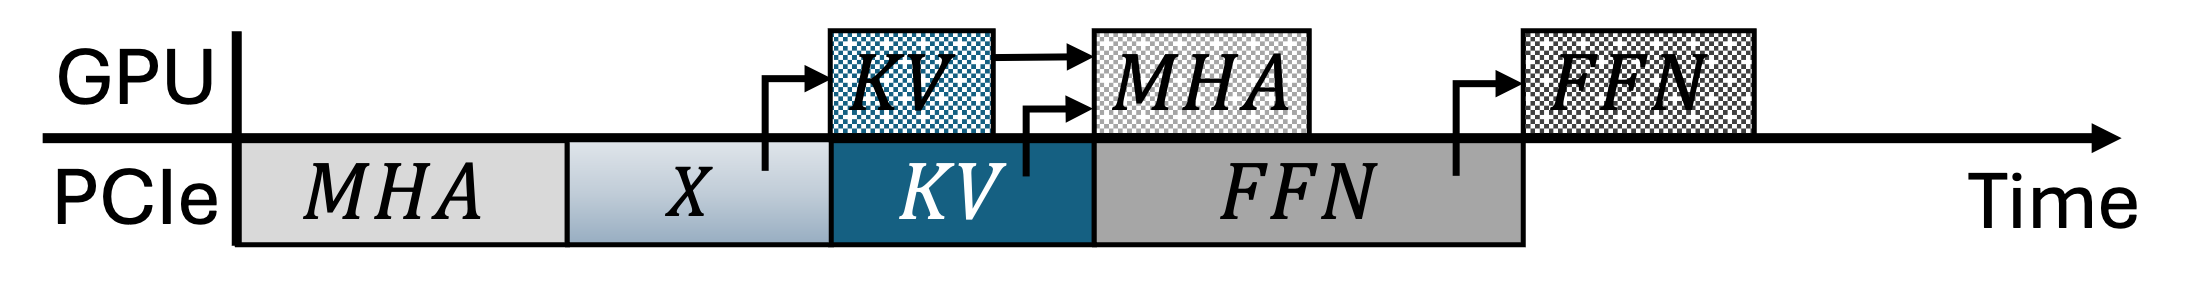
\includegraphics[width=\columnwidth]{assets/3b.png}
    \caption{通过 KV 缓存部分重计算卸载用于行式调度的管道。}
\end{subfigure}

\caption{两种卸载管道的比较。}
\label{fig:row-by-row}
\end{figure}


在 {\paperName}，GPU 不是将整个 KV 缓存从 CPU 内存传输到 GPU 内存，而是使用首先从 CPU 传输的相应输入激活重计算部分 KV 缓存，而剩余的 KV 缓存则异步传输到 GPU，如图所示 \ref{fig:row-by-row}（二）。然后，GPU 将重计算的 KV 缓存与传输的 KV 缓存合并以执行 MHA 计算。 


\noindent \textbf{具有 KV 缓存部分重计算的逐列调度。}
当性能目标是最大化吞吐量时，调度程序模块采用逐列执行计划。这种方法，如图所示 \ref{fig:column-by-column-recomputation}，通过跨多个批次重用模型权重来适应大批量推理。
一旦批次 0 的 KV 缓存完全传输，批次 1 的激活就会被传输。同时，GPU 开始计算批次 0 的 MHA。与逐行调度不同，逐行调度在移至下一个批次之前按顺序处理单个批次内的所有层，而逐列调度则在同一层上处理多个批次。因此，必须存储与重计算的 KV 缓存相对应的激活，直到该批次的生成完成。


\begin{figure}[h]
\centering
    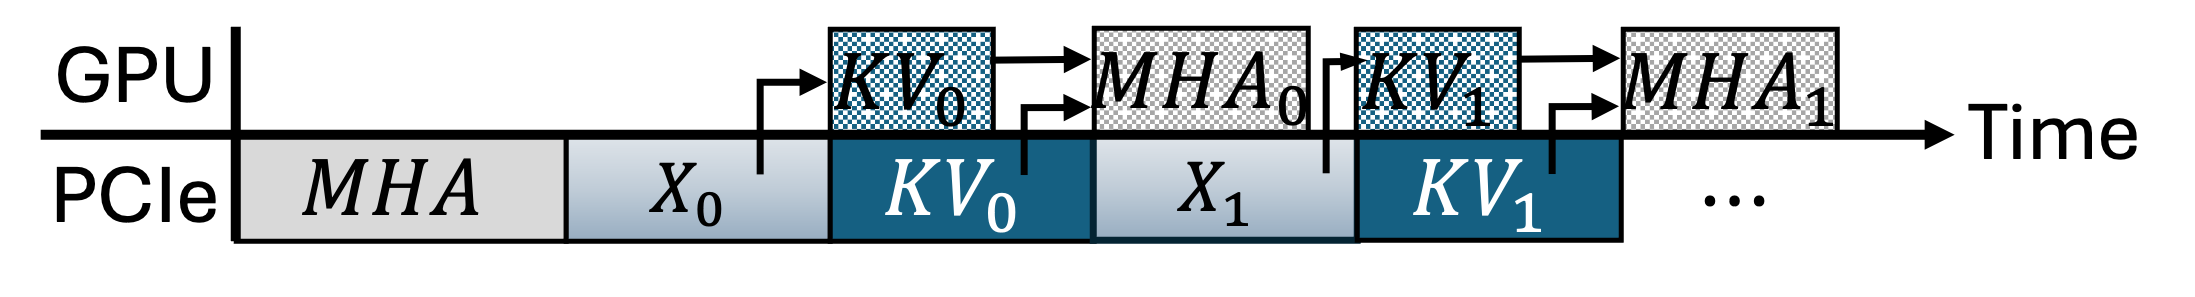
\includegraphics[width=\columnwidth]{assets/4.png}
\caption{通过 KV 缓存部分重计算卸载用于列调度的管道，以最大限度地提高吞吐量。}
\label{fig:column-by-column-recomputation}
\end{figure}

\noindent \textbf{确定最佳 KV 缓存分割点。} 
在这两种调度方法中，目标都是确定最佳分割点，该分割点定义了 KV 缓存在 GPU 上重计算的部分和从 CPU 内存传输的部分之间的划分。该问题可以表述为线性规划问题。
逐行调度可以视为逐列调度的特例，其中不传输用于重计算 KV 缓存的激活。我们首先制定逐列计划的问题，然后演示它如何简化为逐行计划。

给定当前序列长度 $s'$（大于提示长度 $s$），传输到 GPU 的第 $i$ 层激活表示为 $ {X}^i[0:l] $，其中 $0 \leq l \leq s'$。后续 token 的剩余 KV 缓存表示为 $ {K}^i[l:s'] $ 和 $ {V}^i[l:s'] $。这些激活的内存使用量为：
% \begin{align}
% M_{{X}^i[0:l]} &= b \times l \times h \times p, \\
% {M}_{{KV}^i[l:s']} &= 2 \times b \times (s' - l) \times h \times p.
% \end{align}

\begin{equation}
\begin{aligned}
M_{{X}^i[0:l]} &= b \times l \times h \times p, \\
{M}_{{KV}^i[l:s']} &= 2 \times b \times (s' - l) \times h \times p.
\end{aligned}
\end{equation}


\noindent 重计算 KV 缓存 $ {X}^i[0:l] $ 要求：  

\begin{equation}
\begin{aligned}
{K}^i[0:l] &= {X}^i[0:l] \cdot {W}^i_K, \\
{V}^i[0:l] &= {X}^i[0:l] \cdot {W}^i_V.
\end{aligned}
\label{eq:recompute}
\end{equation}

\noindent GPU 上的重计算需要以下浮点运算

\begin{equation}
N_{{KV}^i[0:l]} = 4 \times b \times l \times h^2.
\end{equation}

\noindent 因此，重计算时间 $ t_{gpu}^i $ KV 缓存由下式给出

\begin{equation}
t_{recomp}^i = \frac{N_{{KV}^i[0:l]}}{v_{gpu}},
\end{equation}

\noindent 其中 $ v_{gpu} $ 表示 GPU 处理速度。总处理时间 $ t^i $ 如下： 

\begin{equation}
t^i = \frac{{M}_{{X}^i[0:l]}}{v_{com}} + \max\left(t_{recomp}^i, \frac{{M}_{{KV}^i[l:s']}}{v_{com}}\right),
\label{eq:lp_target}
\end{equation}

\noindent 其中 $ v_{com} $ 表示激活和 KV 缓存的数据传输速度。

目标是确定最优 $ l $ 最大限度地减少总处理时间 $ t^i $，这变成了一个线性规划问题：  

\begin{equation}
\begin{aligned}
\min_{l} \quad & t^i \\
\text{s.t.} \quad & 0 \leq l \leq s \quad \forall i \in \{1, \ldots, n\}.
\end{aligned}
\label{eq:lp}
\end{equation}

最佳分割点 $l$ 取决于当前序列长度 $s'$，它在生成过程中增加，因此必须自适应地确定。幸运的是，解决这一线性规划问题在计算上可以忽略不计，因为只有一个整数变量。若式中第一项~\eqref{eq:lp_target} 被省略，问题就简化为逐行调度。


\subsection{运行时模块} 

\textbf{异步重叠。}
为了实现 GPU 计算和 CPU-GPU 通信的并发执行，运行时模块采用包含六类任务的通信并行策略：权重加载、KV 缓存加载、激活加载、重计算激活加载、KV 缓存存储和激活存储，详见附录 \ref{app:overlapping}。结合双缓冲和预取技术，运行时在处理当前批次的同时，加载下一层权重，取回 KV 缓存重计算所需激活和下一批次的 KV 缓存，并存储上一批次的缓存和激活。 


\noindent \textbf{固定内存。}
与之前的工作一样，优化数据传输 \cite{sheng2023flexgen, yu2024twinpilots}，我们利用固定的 CPU 内存来重计算激活并将权重传输到 GPU。使用固定内存可以实现更快的异步传输，因为它避免了将数据分页进出的需要。


\noindent \textbf{隐藏 KV 缓存部分重计算。}
如果 KV 缓存和模型权重都被卸载，且传输的 KV 缓存小于模型权重大小，那么带 KV 缓存部分重计算的粗粒度计算管道可能会降低推理性能。原因是重计算必须等待所有 MHA 权重（$W_Q$, $W_K$, $W_V$ 和 $W_O$）加载完成，如图 \ref{fig:hiding-recomputation-pipeline}(a) 所示，这会延迟 MHA 计算。然而，KV 缓存重计算只需要 $W_K$ 和 $W_V$（式~\eqref{eq:recompute}），无需等待完整权重加载。为此，我们实现了细粒度 MHA 管道，优先加载 $W_K$ 和 $W_V$。一旦这些权重可用，KV 缓存重计算即可立即开始。如图 \ref{fig:hiding-recomputation-pipeline}(b) 所示，$W_K$ 和 $W_V$ 用于 KV 缓存部分重计算，随后 $W_Q$ 和 $W_O$ 用于 MHA 计算。这种方法有效地将 KV 缓存重计算与权重加载重叠，确保在最坏情况下性能不会低于受权重加载瓶颈限制的基线。



\begin{figure}[h]
\centering
% First subfigure
\begin{subfigure}[t]{\columnwidth}
\centering
    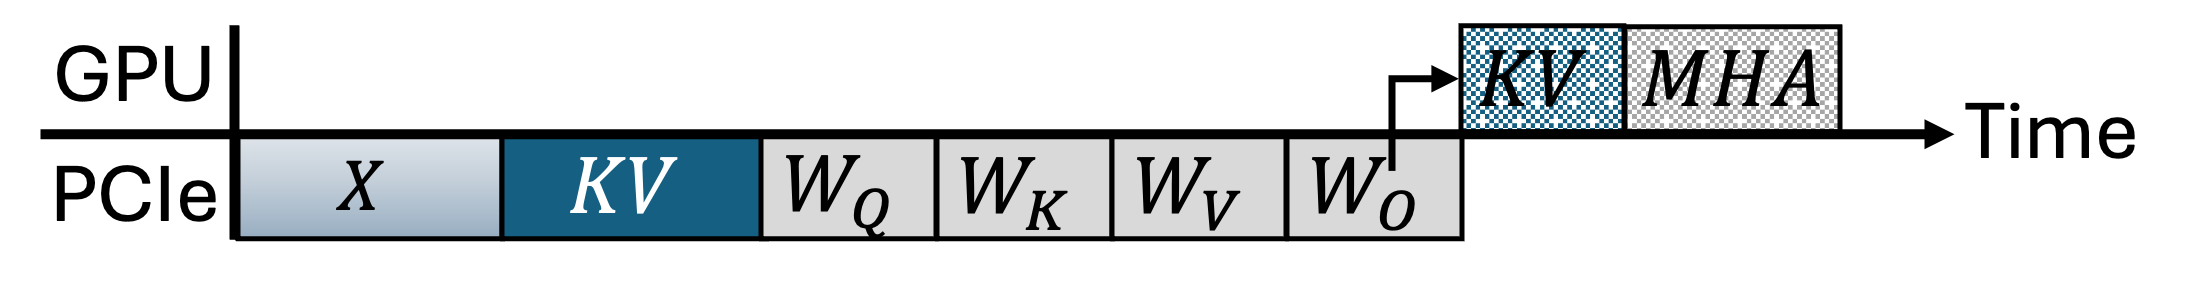
\includegraphics[width=\columnwidth]{assets/5a.png}
\caption{具有延迟 KV 缓存部分重计算的粗粒度卸载管道。}
\end{subfigure}

% Second subfigure
\begin{subfigure}[t]{\columnwidth}
\centering
    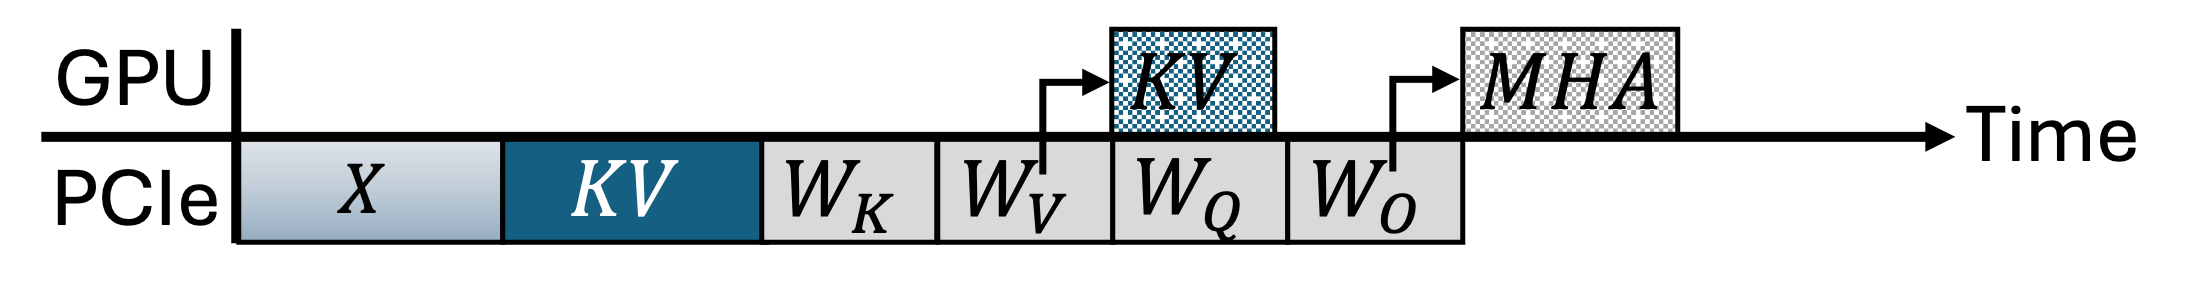
\includegraphics[width=\columnwidth]{assets/5b.png}
\caption{细粒度卸载管道与 KV 缓存重计算和权重加载重叠。}
\end{subfigure}

\caption{MHA层不同粒度的卸载管道比较。}
\label{fig:hiding-recomputation-pipeline}
\end{figure}


\section{实验}
\label{sec:exp}
\textbf{硬件。}
在我们的实验中，我们使用具有 40 GB 内存的 NVIDIA A100 GPU，通过 PCIe 4.0 x16 接口连接到 CPU，提供 32 GB/s 的带宽。 CPU 是 AMD EPYC 处理器，具有 64 核，运行频率为 2.6 GHz。
我们的方法和实现自动适应底层硬件，从而允许跨不同系统架构灵活部署。


\noindent \textbf{模型。}
我们评估 {\paperName} 使用OPT模型 \cite{zhang2022opt} 参数大小范围从 6.7B 到 30B。虽然我们的实验侧重于 OPT 模型，但本工作中提出的重计算技术与其他 LLM 架构兼容，例如 LLaMa \cite{touvron2023llama} 和GPT-3 \cite{brown2020language}，由于它们相似的注意力机制 \cite{ashish2017attention}.

\noindent \textbf{工作量。}
我们评估 {\paperName} 针对两种类型的工作负载：面向延迟的和面向吞吐量的。在面向延迟的工作负载中，模型权重保留在 GPU 内存中，以避免代价高昂的重复加载。由于GPU 内存大小有限，实验使用OPT-6.7B和OPT-13B进行。在面向吞吐量的工作负载中，模型权重在计算后卸载到 CPU，以释放更多 GPU 内存来处理更大的批次。使用 OPT-6.7B、OPT-13B 和 OPT-30B 评估此设置。

为了提供准确的比较，我们使用与 FlexGen 中相同的数据集 \cite{sheng2023flexgen} 提示统一填充为相同的长度，模型配置为每个提示生成 32 或 128 个标记。为了评估不同输入场景的性能，我们的评估使用 256、512 和 1024 个标记的提示长度。性能指标包括面向延迟的工作负载的解码延迟（生成令牌所需的时间）和面向吞吐量的工作负载的解码吞吐量（每秒生成的令牌），如下所示 {\paperName} 不影响预填充性能。我们分别报告五次测试运行的平均解码延迟和吞吐量。

\noindent \textbf{基线。}
在我们的实验中，我们使用 DeepSpeed Inference \cite{aminabadi2022deepspeed}, Hugging Face Accelerate \cite{accelerate} 作为面向延迟的工作负载实验的基准，因为 Hugging Face Transformers 库目前支持 KV 缓存卸载到 CPU 内存，同时仍保留 GPU 内存中的模型权重。我们使用 FlexGen \cite{sheng2023flexgen} 作为面向吞吐量的工作负载实验的基准，因为它通过将模型权重和 KV 缓存卸载到 CPU 来支持逐列调度。

\noindent \textbf{执行。} {\paperName} 在 Hugging Face Transformers (v4.46.1) 之上实现 \cite{wolf2020transformers} 和 FlexGen \cite{sheng2023flexgen} 确保与基线进行公平比较的框架。在 Transformers 实现中，我们利用 GPU 内存中的双缓冲来重叠跨解码器层的 KV 缓存传输。对于 Transformers 和 FlexGen 实现，我们利用 CUDA 流来实现异步重叠，如算法中所述 \ref{alg:block_schedule_overlap}.

\subsection{面向延迟的实验}

\begin{figure*}[t]
\centering
    % Row 1
    \begin{subfigure}[t]{0.32\textwidth}
        \centering
        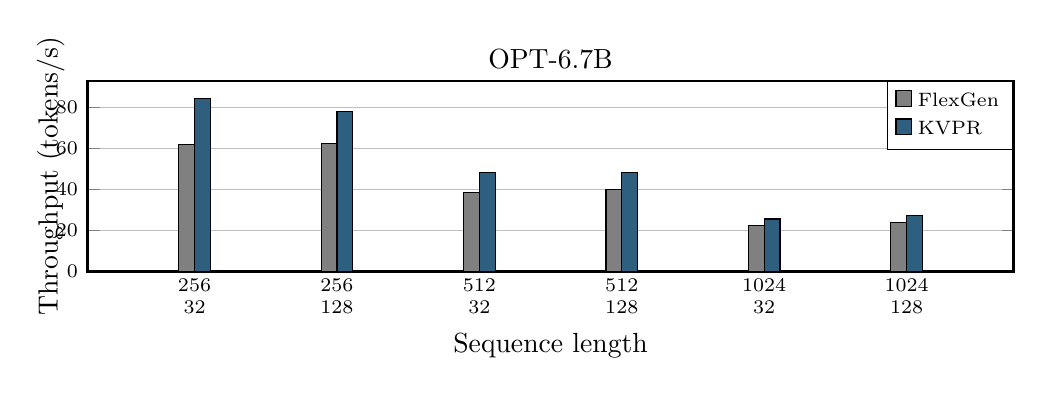
\begin{tikzpicture}
            \begin{axis}[
                axis line style={line width=1pt},
                title={OPT-6.7B},
                title style={yshift=-5pt},
                width=1.1\textwidth,
                height=4cm,
                ybar=0pt,
                bar width=.2cm,
                tick label style={font=\scriptsize},
                symbolic x coords={A, B, C, D, E, F},
                xticklabel style={yshift=5pt, align=center},
                xticklabels={{256 \\ 32}, {256 \\ 128}, {512 \\ 32}, {512 \\ 128}, {1024 \\ 32}, {1024 \\ 128}},
                xtick=data,
                xtick style={draw=none},
                ytick={0, 20, 40, 60, 80},
                ymin=0,
                xlabel={Sequence length},
                ylabel={Throughput (tokens/s)},
                ylabel style={yshift=-10pt},
                enlarge x limits=0.15,
                grid=major,
                grid style=solid,
                major x grid style={draw=none},
                legend entries={FlexGen, {\paperName}},
                legend style={at={(1,1)}, anchor=north east, font=\scriptsize, row sep=0cm, column sep=0cm, legend cell align=left},
                legend image code/.code={\draw[yshift=-0.06cm] rectangle (0.2cm,0.2cm);},
            ]
            \addplot[fill=gray!] coordinates {(A, 62.04) (B, 62.153) (C, 38.307) (D, 39.823) (E, 22.509) (F, 23.886)};
            \addplot[fill=darkteal] coordinates {(A, 84.316) (B, 77.863) (C, 48.213) (D, 48.283) (E, 25.543) (F, 27.396)};
            \end{axis}
        \end{tikzpicture}
    \end{subfigure}
    \begin{subfigure}[t]{0.32\textwidth}
        \centering
        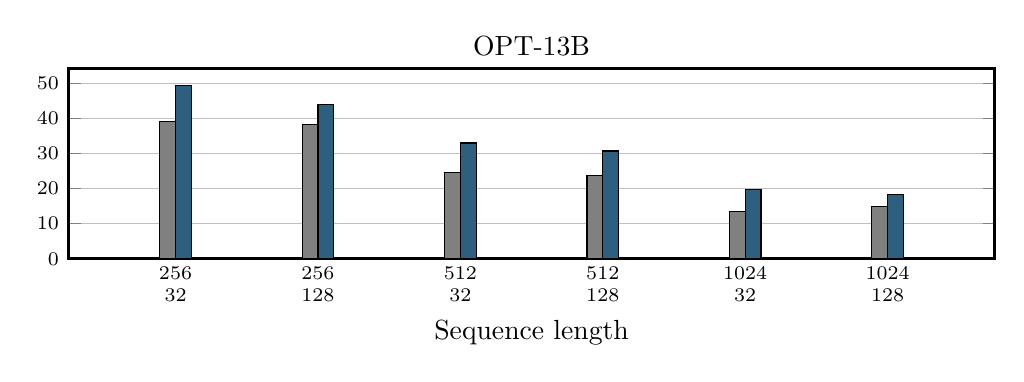
\begin{tikzpicture}
            \begin{axis}[
                axis line style={line width=1pt},
                title={OPT-13B},
                title style={yshift=-5pt},
                width=1.1\textwidth,
                height=4cm,
                ybar=0pt,
                bar width=.2cm,
                tick label style={font=\scriptsize},
                symbolic x coords={A, B, C, D, E, F},
                xticklabel style={yshift=5pt, align=center},
                xticklabels={{256 \\ 32}, {256 \\ 128}, {512 \\ 32}, {512 \\ 128}, {1024 \\ 32}, {1024 \\ 128}},
                xtick=data,
                xtick style={draw=none},
                ytick={0, 10, 20, 30, 40, 50},
                ymin=0,
                xlabel={Sequence length},
                enlarge x limits=0.15,
                grid=major,
                grid style=solid,
                major x grid style={draw=none},
            ]
            \addplot[fill=gray!] coordinates {(A, 39.096) (B, 38.339) (C, 24.659) (D, 23.832) (E, 13.582) (F, 14.997)};
            \addplot[fill=darkteal] coordinates {(A, 49.418) (B, 44.022) (C, 33.054) (D, 30.76) (E, 19.817) (F, 18.364)};
            \end{axis}
        \end{tikzpicture}
    \end{subfigure}
    % \hfill
    \begin{subfigure}[t]{0.32\textwidth}
        \centering
        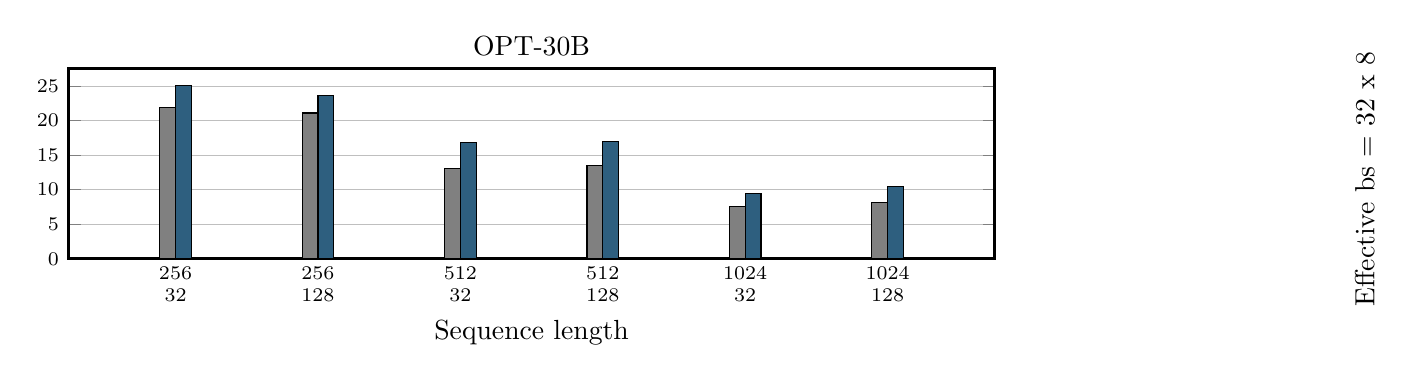
\begin{tikzpicture}
            \begin{axis}[
                axis line style={line width=1pt},
                title={OPT-30B},
                title style={yshift=-5pt},
                width=1.1\textwidth,
                height=4cm,
                ybar=0pt,
                bar width=.2cm,
                tick label style={font=\scriptsize},
                symbolic x coords={A, B, C, D, E, F},
                xticklabel style={yshift=5pt, align=center},
                xticklabels={{256 \\ 32}, {256 \\ 128}, {512 \\ 32}, {512 \\ 128}, {1024 \\ 32}, {1024 \\ 128}},
                xtick=data,
                xtick style={draw=none},
                ytick={0, 5, 10, 15, 20, 25},
                ymin=0,
                xlabel={Sequence length},
                ylabel style={at={(1.4,-0.3)}, anchor=west},
                ylabel={Effective bs = 32 x 8},
                enlarge x limits=0.15,
                grid=major,
                grid style=solid,
                major x grid style={draw=none},
            ]
            \addplot[fill=gray!] coordinates {(A, 21.912) (B, 21.108) (C, 13.096) (D, 13.479) (E, 7.61) (F, 8.127)};
            \addplot[fill=darkteal] coordinates {(A, 25.064) (B, 23.692) (C, 16.829) (D, 16.917) (E, 9.456) (F, 10.485)};
            \end{axis}
        \end{tikzpicture}
    \end{subfigure}
    % Row 2
    \begin{subfigure}[t]{0.32\textwidth}
        \centering
        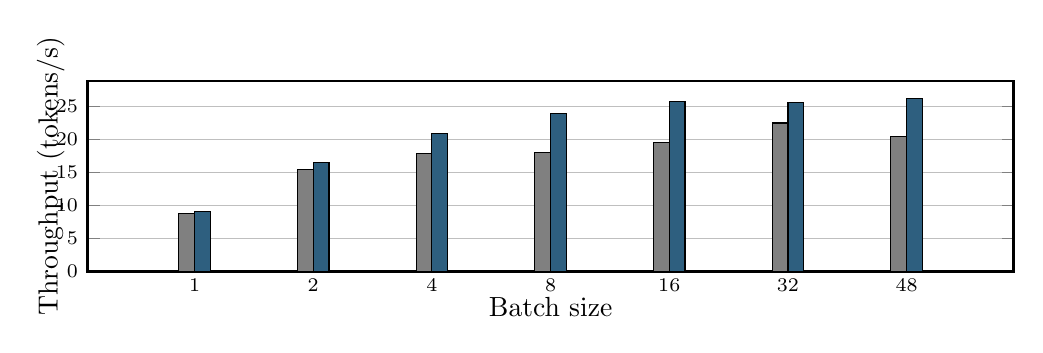
\begin{tikzpicture}
            \begin{axis}[
                axis line style={line width=1pt},
                width=1.1\textwidth,
                height=4cm,
                ybar=0pt,
                bar width=.2cm,
                tick label style={font=\scriptsize},
                symbolic x coords={A, B, C, D, E, F, G},
                xticklabel style={yshift=5pt, align=center},
                xticklabels={1, 2, 4, 8, 16, 32, 48},
                xtick=data,
                xtick style={draw=none},
                ytick={0, 5, 10, 15, 20, 25},
                ymin=0,
                xlabel={Batch size},
                xlabel style={yshift=5pt},
                ylabel={Throughput (tokens/s)},
                ylabel style={yshift=-10pt},
                enlarge x limits=0.15,
                grid=major,
                grid style=solid,
                major x grid style={draw=none},
            ]
            \addplot[fill=gray!] coordinates {(A, 8.799) (B, 15.393) (C, 17.89) (D, 18.075) (E, 19.521) (F, 22.509) (G, 20.435)};
            \addplot[fill=darkteal] coordinates {(A, 9.046) (B, 16.573) (C, 20.895) (D, 23.941) (E, 25.712) (F, 25.543) (G, 26.241)};
            \end{axis}
        \end{tikzpicture}
    \end{subfigure}
    % \hfill
    \begin{subfigure}[t]{0.32\textwidth}
        \centering
        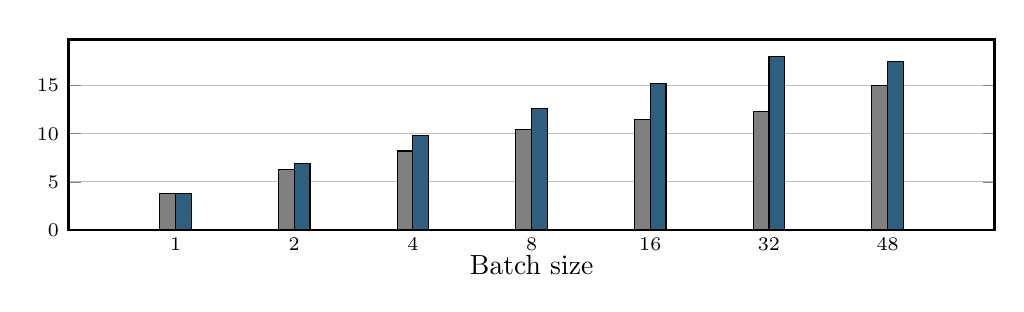
\begin{tikzpicture}
            \begin{axis}[
                axis line style={line width=1pt},
                width=1.1\textwidth,
                height=4cm,
                ybar=0pt,
                bar width=.2cm,
                tick label style={font=\scriptsize},
                symbolic x coords={A, B, C, D, E, F, G},
                xticklabel style={yshift=5pt, align=center},
                xticklabels={1, 2, 4, 8, 16, 32, 48},
                xtick=data,
                xtick style={draw=none},
                ytick={0, 5, 10, 15, 20},
                ymin=0,
                xlabel={Batch size},
                xlabel style={yshift=5pt},
                ylabel style={yshift=-10pt},
                enlarge x limits=0.15,
                grid=major,
                grid style=solid,
                major x grid style={draw=none},
            ]
            \addplot[fill=gray!] coordinates {(A, 3.827) (B, 6.263) (C, 8.211) (D, 10.455) (E, 11.507) (F, 12.313) (G, 15.027)};
            \addplot[fill=darkteal] coordinates {(A, 3.821) (B, 6.908) (C, 9.835) (D, 12.621) (E, 15.248) (F, 18.007) (G, 17.55)};
            \end{axis}
        \end{tikzpicture}
    \end{subfigure}
    % \hfill
    \begin{subfigure}[t]{0.32\textwidth}
        \centering
        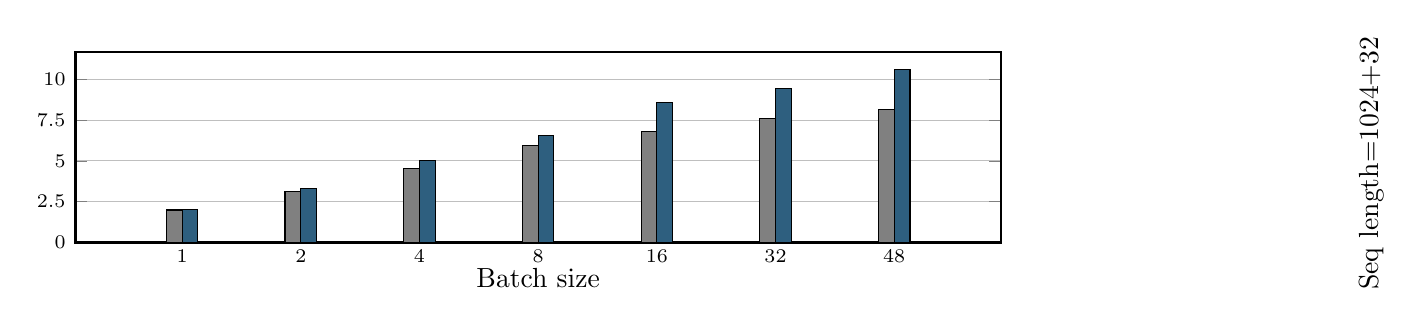
\begin{tikzpicture}
            \begin{axis}[
                axis line style={line width=1pt},
                width=1.1\textwidth,
                height=4cm,
                ybar=0pt,
                bar width=.2cm,
                tick label style={font=\scriptsize},
                symbolic x coords={A, B, C, D, E, F, G},
                xticklabel style={yshift=5pt, align=center},
                xticklabels={1, 2, 4, 8, 16, 32, 48},
                xtick=data,
                xtick style={draw=none},
                ytick={0, 2.5, 5, 7.5, 10},
                ymin=0,
                xlabel={Batch size},
                xlabel style={yshift=5pt},
                ylabel style={at={(1.4,-0.3)}, anchor=west},
                ylabel={Seq length=1024+32},
                enlarge x limits=0.15,
                grid=major,
                grid style=solid,
                major x grid style={draw=none},
            ]
            \addplot[fill=gray!] coordinates {(A, 1.989) (B, 3.1) (C, 4.56) (D, 5.935) (E, 6.785) (F, 7.61) (G, 8.172)};
            \addplot[fill=darkteal] coordinates {(A, 2.012) (B, 3.318) (C, 5.009) (D, 6.544) (E, 8.567) (F, 9.456) (G, 10.613)};
            \end{axis}
        \end{tikzpicture}
    \end{subfigure}

    \caption{各种型号和配置的吞吐量比较。}
    \label{fig:throughput_exp}
\end{figure*}

我们评估不同序列长度设置完成单个批次所需的解码延迟。图 \ref{fig:latency-exp} 表明 {\paperName} 对于 OPT-6.7B 和 OPT-13B，其性能始终优于基准、DeepSpeed Inference 和 Hugging Face Accelerate。 
实验结果表明 {\paperName} 减少解码延迟，尤其是在较长的生成长度下。例如，OPT 6.7B，提示长度为 128，生成 128 个令牌，延迟减少约 35.8\% 与Hugging Face Accelerate相比。附录中提供了详细的实验结果，包括 KV 缓存大小、GPU 峰值内存使用情况以及生成过程中的最佳重计算分割点 \ref{app:detailed-exp} 和 \ref{app:optimal-split-points}. 

\begin{figure}[h]
    \centering
    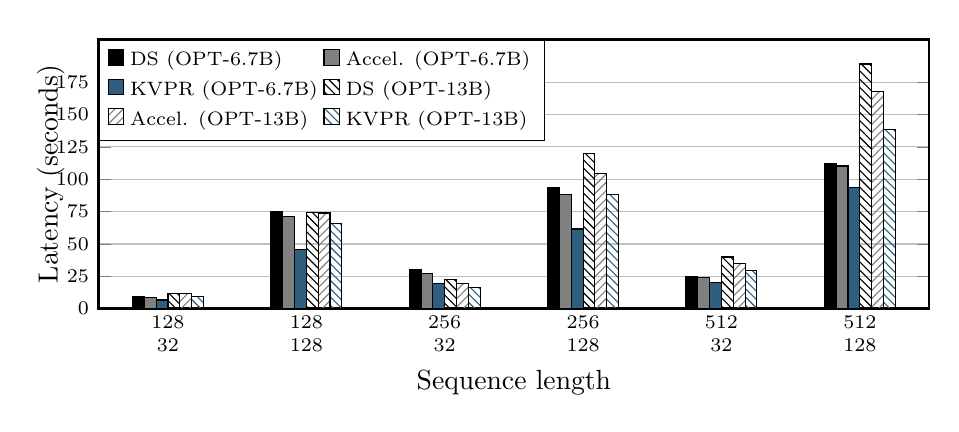
\begin{tikzpicture}
        \begin{axis}[
            axis line style={line width=1pt},
            width=\columnwidth,
            height=5cm,
            ybar=0pt,
            bar width=.15cm,
            tick label style={font=\scriptsize},
            symbolic x coords={A, B, C, D, E, F},
            xticklabel style={align=center},
            xticklabels={{128 \\ 32}, {128 \\ 128}, {256 \\ 32}, {256 \\ 128}, {512 \\ 32}, {512 \\ 128}},
            xtick=data,
            xtick style={draw=none},
            xticklabel style={yshift=5pt, align=center},
            xlabel={Sequence length},
            ylabel={Latency (seconds)},
            ylabel style={yshift=-10pt},
            ymin=0,
            ytick={0, 25, 50, 75, 100, 125, 150, 175},
            grid=major,
            grid style=solid,
            major x grid style={draw=none},
            legend entries={DS (OPT-6.7B), Accel. (OPT-6.7B), {\paperName} (OPT-6.7B), DS (OPT-13B), Accel. (OPT-13B), {\paperName} (OPT-13B)},
            legend style={at={(0,1)}, anchor=north west, font=\scriptsize, row sep=0cm, column sep=0cm, legend cell align=left, legend columns=2},
            legend image code/.code={\draw[yshift=-0.06cm] rectangle (0.2cm,0.2cm);},
        ]

        % DS (6.7B)
        \addplot[fill=black] coordinates {(A,9.613) (B,74.805) (C,29.892) (D,93.965) (E,25.162) (F,112.516)};

        % HF (6.7B)
        \addplot[fill=gray] coordinates {(A,8.905) (B,71.327) (C,26.825) (D,88.354) (E,24.390) (F,110.277)};

        % Ours (6.7B)
        \addplot[fill=darkteal] coordinates {(A,6.651) (B,45.766) (C,19.138) (D,61.597) (E,20.349) (F,93.932)};

        % DS (13B)
        \addplot[pattern=north west lines, pattern color=black] coordinates {(A,11.525) (B,74.015) (C,22.740) (D,119.806) (E,39.956) (F,189.124)};

        % HF (13B)
        \addplot[pattern=north east lines, pattern color=gray] coordinates {(A,11.409) (B,73.896) (C,19.381) (D,104.115) (E,35.066) (F,168.155)};

        % Ours (13B)
        \addplot[pattern=north west lines, pattern color=darkteal] coordinates {(A,9.148) (B,66.119) (C,16.654) (D,88.492) (E,29.215) (F,138.377)};

        \end{axis}
    \end{tikzpicture}
    \caption{批量大小为 64 时，不同序列长度下单批次解码延迟。}
    \label{fig:latency-exp}
\end{figure}


\subsection{面向吞吐量的实验}



我们还评估解码阶段的吞吐量性能，如下所示 {\paperName} 不影响预填充阶段。为了最大化吞吐量，我们将有效批量大小设置为 32 x 8，这意味着每个层在移动到下一层之前按顺序计算 8 个大小为 32 的批量。图第一行 \ref{fig:throughput_exp} 显示结果，证明 {\paperName} 在不同模型的所有序列长度设置下，其性能始终优于 FlexGen。最高可达15.1\%, 46.2\%和 29.0\% 分别提高了 OPT-6.7B、OPT-13B 和 OPT-30B 的吞吐量。附录中提供了低端 GPU 系统上的其他实验结果 \ref{app:low-end-gpu-experiments}。

我们也比较 {\paperName} 使用 FlexGen，批量大小从 1 到 48 不等，固定提示长度为 1,024，生成长度为 32，如图第二行所示 \ref{fig:throughput_exp}. {\paperName} 在所有批量大小上始终优于 FlexGen。随着KV 缓存变大， {\paperName} 由于减少了 PCIe 总线上的 KV 缓存传输，显示出更大的性能优势。



\subsection{GPU利用率}

\noindent 为了评估效率的提高，我们分析了时间资源利用率 {\paperName} 和FlexGen如图所示 \ref{fig:ablation-utilization}。首先在预填充阶段，两种方法都达到了 GPU 的充分利用，因为预填充阶段是计算密集型的。然而，在解码阶段，与FlexGen相比， {\paperName} 提高 GPU 利用率，从 85 增加到\% 至 99\% 平均而言，通过将 GPU 计算与 CPU-GPU 数据传输重叠，同时保持黑线所示的相同峰值内存使用量。

\begin{figure}[h]
\centering
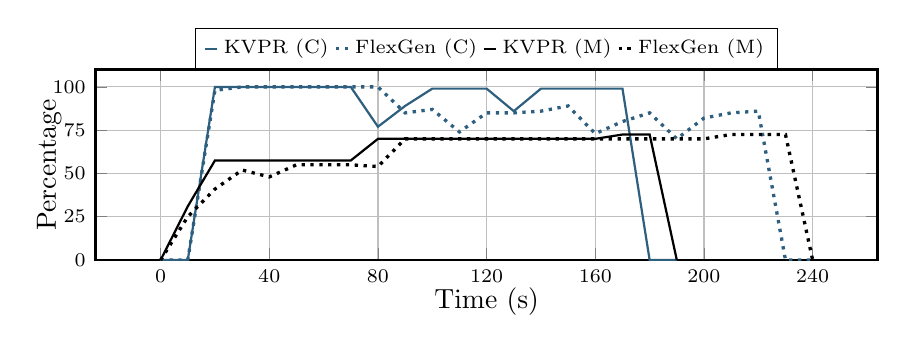
\begin{tikzpicture}
    \begin{axis}[
        axis line style={line width=1pt},
        width=0.95\columnwidth,
        height=4cm,
        tick label style={font=\scriptsize},
        xlabel={Time (s)},
        xlabel style={yshift=5pt},
        ylabel={Percentage},
        ylabel style={yshift=-10pt},
        ymin=0, ymax=110,
        xtick={0,40,80,120,160,200,240},
        ytick={0,25,50,75,100},
        grid=major,
        legend entries={{\paperName} (C), FlexGen (C), {\paperName} (M), FlexGen (M)},
        legend style={at={(0.5, 1)}, anchor=south, font=\scriptsize, column sep=0cm, legend cell align=left, legend columns=4},
        legend image post style={xscale=0.26}
    ]

        % Our Method Compute Usage (Solid)
        \addplot[solid, color=darkteal, thick] coordinates {
            (0, 0) (10, 0) (20, 100) (30, 100) (40, 100) (50, 100) 
            (60, 100) (70, 100) (80, 77) (90, 89) (100, 99) (110, 99) 
            (120, 99) (130, 86) (140, 99) (150, 99) (160, 99) (170, 99) 
            (180, 0) (190, 0)
        };
        
        % FlexGen Compute Usage (Dotted)
        \addplot[dotted, color=darkteal, very thick] coordinates {
            (0, 0) (10, 0) (20, 98) (30, 100) (40, 100) (50, 100) 
            (60, 100) (70, 100) (80, 100) (90, 85) (100, 87) (110, 74) 
            (120, 85) (130, 85) (140, 86) (150, 89) (160, 73) (170, 80) 
            (180, 85) (190, 70) (200, 82) (210, 85) (220, 86) (230, 0) 
            (240, 0)
        };

        % Our Method Memory Usage (Solid)
        \addplot[solid, color=black, thick] coordinates {
            (0, 0) (10, 31) (20, 57.5) (30, 57.5) (40, 57.5) (50, 57.5) 
            (60, 57.5) (70, 57.5) (80, 70) (90, 70) (100, 70) (110, 70) 
            (120, 70) (130, 70) (140, 70) (150, 70) (160, 70) (170, 72.5) 
            (180, 72.5) (190, 0)
        };

        % FlexGen Memory Usage (Dotted)
        \addplot[dotted, color=black, very thick] coordinates {
            (0, 0) (10, 25) (20, 41) (30, 52) (40, 48) (50, 55) 
            (60, 55) (70, 55) (80, 54) (90, 70) (100, 70) (110, 70) 
            (120, 70) (130, 70) (140, 70) (150, 70) (160, 70) (170, 70) 
            (180, 70) (190, 70) (200, 70) (210, 72.5) (220, 72.5) 
            (230, 72.5) (240, 0)
        };

    \end{axis}
\end{tikzpicture}
\caption{{\paperName} 与 FlexGen 在解码阶段的计算和内存资源使用情况。}
\label{fig:ablation-utilization}
\end{figure}


\subsection{KV 缓存压缩}

我们应用分组 4 位量化来压缩 KV 缓存，这已被证明对模型精度的影响最小 \cite{sheng2023flexgen}。图 \ref{fig:compression} 表明应用压缩减少了传输到 GPU 的数据量，从而进一步提高了解码吞吐量。这些结果展示了兼容性 {\paperName} KV 缓存压缩及其通过缓解 PCIe 带宽瓶颈实现额外性能提升的潜力。

\begin{figure}[h]
\centering
    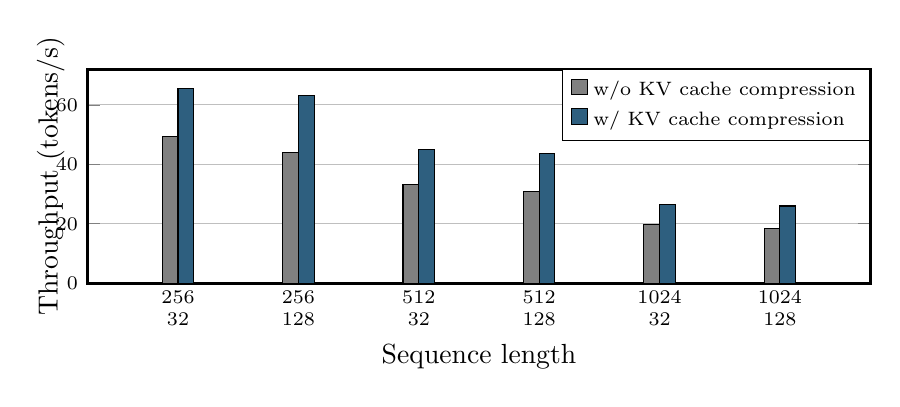
\begin{tikzpicture}
        \begin{axis}[
            axis line style={line width=1pt},
            % title={OPT-13B},
            width=0.95\columnwidth,
            height=4.3cm,
            ybar=0pt,
            bar width=.2cm,
            tick label style={font=\scriptsize},
            symbolic x coords={A, B, C, D, E, F},
            xticklabel style={align=center},
            xticklabels={{256 \\ 32}, {256 \\ 128}, {512 \\ 32}, {512 \\ 128}, {1024 \\ 32}, {1024 \\ 128}},
            xtick=data,
            xtick style={draw=none},
            xticklabel style={yshift=5pt, align=center},
            xlabel={Sequence length},
            ylabel={Throughput (tokens/s)},
            ylabel style={yshift=-10pt},
            ymin=0,
            enlarge x limits=0.15,
            grid=major,
            grid style=solid,
            major x grid style={draw=none},
            legend entries={w/o KV cache compression, w/ KV cache compression},
            legend style={at={(1,1)}, anchor=north east, font=\scriptsize, row sep=0cm, column sep=0cm, legend cell align=left},
            legend image code/.code={\draw[yshift=-0.06cm] rectangle (0.2cm,0.2cm);},
        ]
    \addplot[fill=gray] coordinates {(A, 49.418) (B, 44.022) (C, 33.054) (D, 30.76) (E, 19.817) (F, 18.364)};
    \addplot[fill=darkteal] coordinates {(A, 65.423) (B, 63.098) (C, 45.054) (D, 43.502) (E, 26.537) (F, 25.969)};
    \end{axis}
    \end{tikzpicture}
\caption{通过在 OPT-13B 模型上启用 KV 缓存压缩来提高解码吞吐量。}
\label{fig:compression}
\end{figure}



\subsection{消融研究}

\textbf{隐藏 KV 缓存部分重计算。}
为了评估将 KV 缓存重计算与权重加载重叠的细粒度卸载管道的有效性，我们使用 OPT-6.7B 模型进行了实验。在此消融中，我们使用较小的 KV 缓存大小来确保 MHA 权重始终晚于 KV 缓存到达 GPU。
表 \ref{tab:ablation-hiding} 展示了较小批量大小下的解码延迟，并比较三种配置：FlexGen、不隐藏 KV 缓存重计算的 {\paperName}，以及隐藏 KV 缓存重计算的 {\paperName}。当 batch size 为 1 且 KV 缓存最小时，FlexGen 可以优于不隐藏重计算的 {\paperName}。
通过将 MHA 权重传输与 KV 缓存重计算重叠，{\paperName} 可确保在该场景下性能不低于 FlexGen，尤其是在权重加载是主要瓶颈时。该结果表明，{\paperName} 同时适用于小批量和大批量设置，从而为提升解码性能提供统一方法。 



\begin{table}[h]
\centering
\resizebox{\columnwidth}{!}{%
\begin{tabular}{lcccccc}
\hline
\textbf{Batch size} & \textbf{1} & \textbf{2} & \textbf{4} & \textbf{8} & \textbf{16} & \textbf{32} \\ \hline
KV cache (MB) & 3 & 6 & 12 & 24  & 48  & 64 \\ \hline
FlexGen & \multicolumn{1}{c}{} 1.761 & 3.488 & 6.646 & 12.826 & 23.795 & 41.210 \\ \hline
\begin{tabular}[c]{@{}l@{}}{\paperName} (w/o. hiding \\  KV recomputation)\end{tabular} & \multicolumn{1}{c}{} 1.749 & 3.461 & \textbf{6.766} & 12.930 & 23.613 & 43.462 \\ \hline
\begin{tabular}[c]{@{}l@{}}{\paperName} (w. hiding \\ KV recomputation)\end{tabular} & \multicolumn{1}{c}{} \textbf{1.774} & \textbf{3.586} & 6.696 & \textbf{12.986} & \textbf{24.557} & \textbf{43.945}  \\ \hline
\end{tabular}%
}
\caption{OPT-6.7B 模型的提示长度和生成长度分别为 256 和 64。每个 MHA 块（$W_Q$, $W_K$, $W_V$， 和 $W_O$）需要 128 MB 内存。}
\label{tab:ablation-hiding}
\end{table}




\noindent \textbf{运行时细分。}
图 \ref{fig:ablation-runtime} 给出了 {\paperName} 和 FlexGen 在解码阶段的 MHA 块运行时细分。{\paperName} 将 KV 缓存传输时间从 58\% 显著降低到 38\%，激活传输仅占总运行时间的 8\%。通过基于传输的激活重计算部分 KV 缓存，GPU 计算时间从 2.3\% 增加到 13.3\%。这表明 {\paperName} 能有效重叠 GPU 计算与 CPU-GPU 通信，大幅减少 CPU 到 GPU 的数据传输量，缓解限制 LLM 推理性能的 PCIe 瓶颈。


\begin{figure}[h]
\centering
    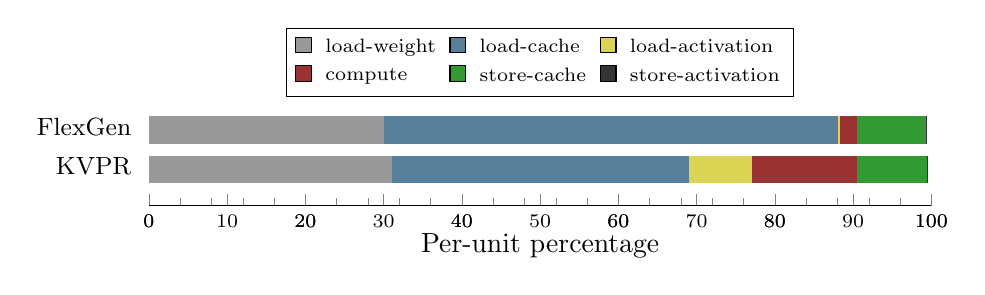
\begin{tikzpicture}
    \node[anchor=east] at (-0.1,1.0) {\small FlexGen};
    \node[anchor=east] at (-0.1,0.5) {\small {\paperName}};

    % Draw stacked bars
    \begin{axis}[
        xbar stacked,
        bar width=10pt,
        width=0.95\columnwidth, 
        height=2.5cm,
        tick label style={font=\scriptsize},
        ytick=data,
        xtick={0,20,40,60,80,100},
        minor x tick num=4,
        xlabel={Per-unit percentage},
        xlabel style={yshift=5pt},
        xmin=0, xmax=100,
        enlarge y limits=0.5,
        axis x line*=bottom,
        axis y line=none,
        every axis plot/.append style={fill opacity=0.8, draw=none},
        legend entries={load-weight, load-cache, load-activation, compute, store-cache, store-activation},
        legend style={at={(0.5, 1.5)}, anchor=south, font=\scriptsize, row sep=0cm, column sep=0.1cm, legend columns=3, legend cell align=left},
        legend image code/.code={\draw[yshift=-0.06cm] rectangle (0.2cm,0.2cm);},
        ]

        \addplot[fill=gray] coordinates {(31,1)}; % load-weight
        \addplot[fill=darkteal] coordinates {(38,1)}; % load-cache
        \addplot[fill=yellow!80!black] coordinates {(8.12,1)}; % load-activation
        \addplot[fill=red!50!black] coordinates {(13.32,1)}; % compute
        \addplot[fill=green!50!black] coordinates {(8.98,1)}; % store-cache
        \addplot[fill=black] coordinates {(0.20,1)}; % store-activation
    \end{axis}

    \begin{axis}[
        xbar stacked,
        bar width=10pt,
        width=0.95\columnwidth, 
        height=3.5cm,
        ytick=data,
        tick label style={font=\scriptsize},
        xmin=0, xmax=100,
        enlarge y limits=0.5,
        axis x line*=bottom,
        axis y line=none,
        every axis plot/.append style={fill opacity=0.8, draw=none},
        ]
        \addplot[fill=gray] coordinates {(30,1)};
        \addplot[fill=darkteal] coordinates {(58,1)};
        \addplot[fill=yellow!80!black] coordinates {(0.254,1)};
        \addplot[fill=red!50!black] coordinates {(2.28,1)};
        \addplot[fill=green!50!black] coordinates {(8.73,1)};
        \addplot[fill=black] coordinates {(0.19,1)};
    \end{axis}

    \end{tikzpicture}

\caption{运行时细分 {\paperName} 和 FlexGen。}
\label{fig:ablation-runtime}
\end{figure}





\section{相关工作}

为满足资源受限环境中的 LLM 内存需求，卸载技术旨在尽量降低 CPU 与 GPU 之间的数据传输延迟。FlexGen \cite{sheng2023flexgen} 将权重、激活和 KV 缓存卸载到 CPU 内存或外部存储，并将优化表述为图遍历问题，以最大化大批量场景下的吞吐量。HeteGen \cite{zhao2024hetegen} 使用 CPU 对卸载权重执行部分计算，同时将剩余工作负载交给 GPU。TwinPilots \cite{yu2024twinpilots} 在算子层面进一步优化 CPU 与 GPU 之间的工作负载平衡。 
% PowerInfer \cite{song2024powerinfer} leverages activation sparsity, offloading infrequently used neurons to the CPU for storage and computation. 
FastDecode \cite{he2024fastdecode} 通过将 KV 缓存和注意力计算完全卸载到 CPU 来减少 KV 缓存数据移动。 
% InstInfer \cite{pan2024instinfer} minimizes inference costs by utilizing computational SSDs for offloading. 
\citeauthor{park2024improving} 和 NEO \cite{jiang2024neo} 将 GPU 线性投影计算与跨多个批次的 CPU 侧注意力计算重叠，以提高资源利用率。

ALISA \cite{zhao2024alisa} 基于稀疏性压缩 KV 缓存，并卸载超出 GPU 显存容量的 KV 缓存。在将 KV 缓存加载到 GPU 时，ALISA 会先重计算一部分 KV 缓存，再传输剩余部分；本文则通过自适应确定最佳切分点，使重计算和传输充分重叠。此外，ALISA 仅处理逐行调度，而 {\paperName} 扩展到了逐列调度。
{\paperName} 与 CPU 辅助方法和 KV 缓存压缩方法正交，因此可以与这些技术结合，进一步提升整体系统性能。附录 \ref{app:comparing-cpu} 的额外实验表明，在某些分布式系统配置中 CPU 可能成为瓶颈。相比之下，{\paperName} 优化 GPU 利用率和数据传输效率，无需依赖额外 CPU 资源，也不需要对 KV 缓存做近似。



\section{结论}

本文提出 \paperName，一种高效的 CPU-GPU I/O 感知 LLM 推理方法，用于加速 KV 缓存加载。{\paperName} 通过 KV 缓存部分重计算减少 CPU 与 GPU 之间的数据传输。通过将该重计算与数据传输重叠，{\paperName} 显著减少 GPU 空闲时间并提升整体推理性能。未来工作可以将该方法扩展到从远程网络存储加载 KV 缓存的场景，或扩展到大规模多 GPU 基础设施，从而进一步提升其适用性和性能。

\section{局限性}
我们的研究代表了通过利用 KV 缓存部分重计算来优化 LLM 推理效率的重要一步。然而， {\paperName} 有一定的局限性，为未来的研究指明了方向。
首先，我们的方法目前仅限于单 GPU 和数据并行多 GPU 推理。它尚未扩展到高级分布式系统，例如模型或张量并行性。将这种方法扩展到这些范例可以支持更大的模型尺寸。
其次，虽然我们解决了 CPU-GPU 通信中的 PCIe 带宽瓶颈，但没有考虑从磁盘或网络存储加载 KV 缓存的场景。尽管如此，{\paperName} 仍可被调整用于加速此类设置中的预填充阶段。
第三，当前的实现仅在推理开始时执行系统分析，并在整个过程中假设静态硬件条件。结合动态分析和运行时自适应优化可以增强该方法的稳健性和效率，特别是在异构或多租户环境中。

\section{致谢}
我们衷心感谢所有审稿人的宝贵时间和建设性意见。本材料基于 NSF 奖项号 2224319、REAL@USC-Meta 中心和 VMware 礼品支持的工作。所表达的观点、意见和/或调查结果属于作者的观点、意见和/或调查结果，不应被解释为代表美国政府的官方观点或政策。

% Bibliography entries for the entire Anthology, followed by custom entries
%\bibliography{anthology,custom}
% Custom bibliography entries only

\bibliography{custom}

\clearpage
\appendix
\section{附录}

\subsection{调度方法}
\label{app:schedule}

图 \ref{app:fig:schedule-methods} 说明了从三层模型生成 2 个标记的两个解码计划（$L_0$, $L_1$， 和 $L_2$）在解码阶段。图中 \ref{app:fig:schedule-methods}(a)，逐行调度在移动到下一个批次之前跨所有层处理每个批次。 
相比之下，图 \ref{app:fig:schedule-methods}(b) 显示了逐列计划，其中每一层在移动到下一层之前都被重用来处理一组批次。


\begin{figure}[h]
\centering
\begin{subfigure}[t]{0.9\columnwidth}
\centering
    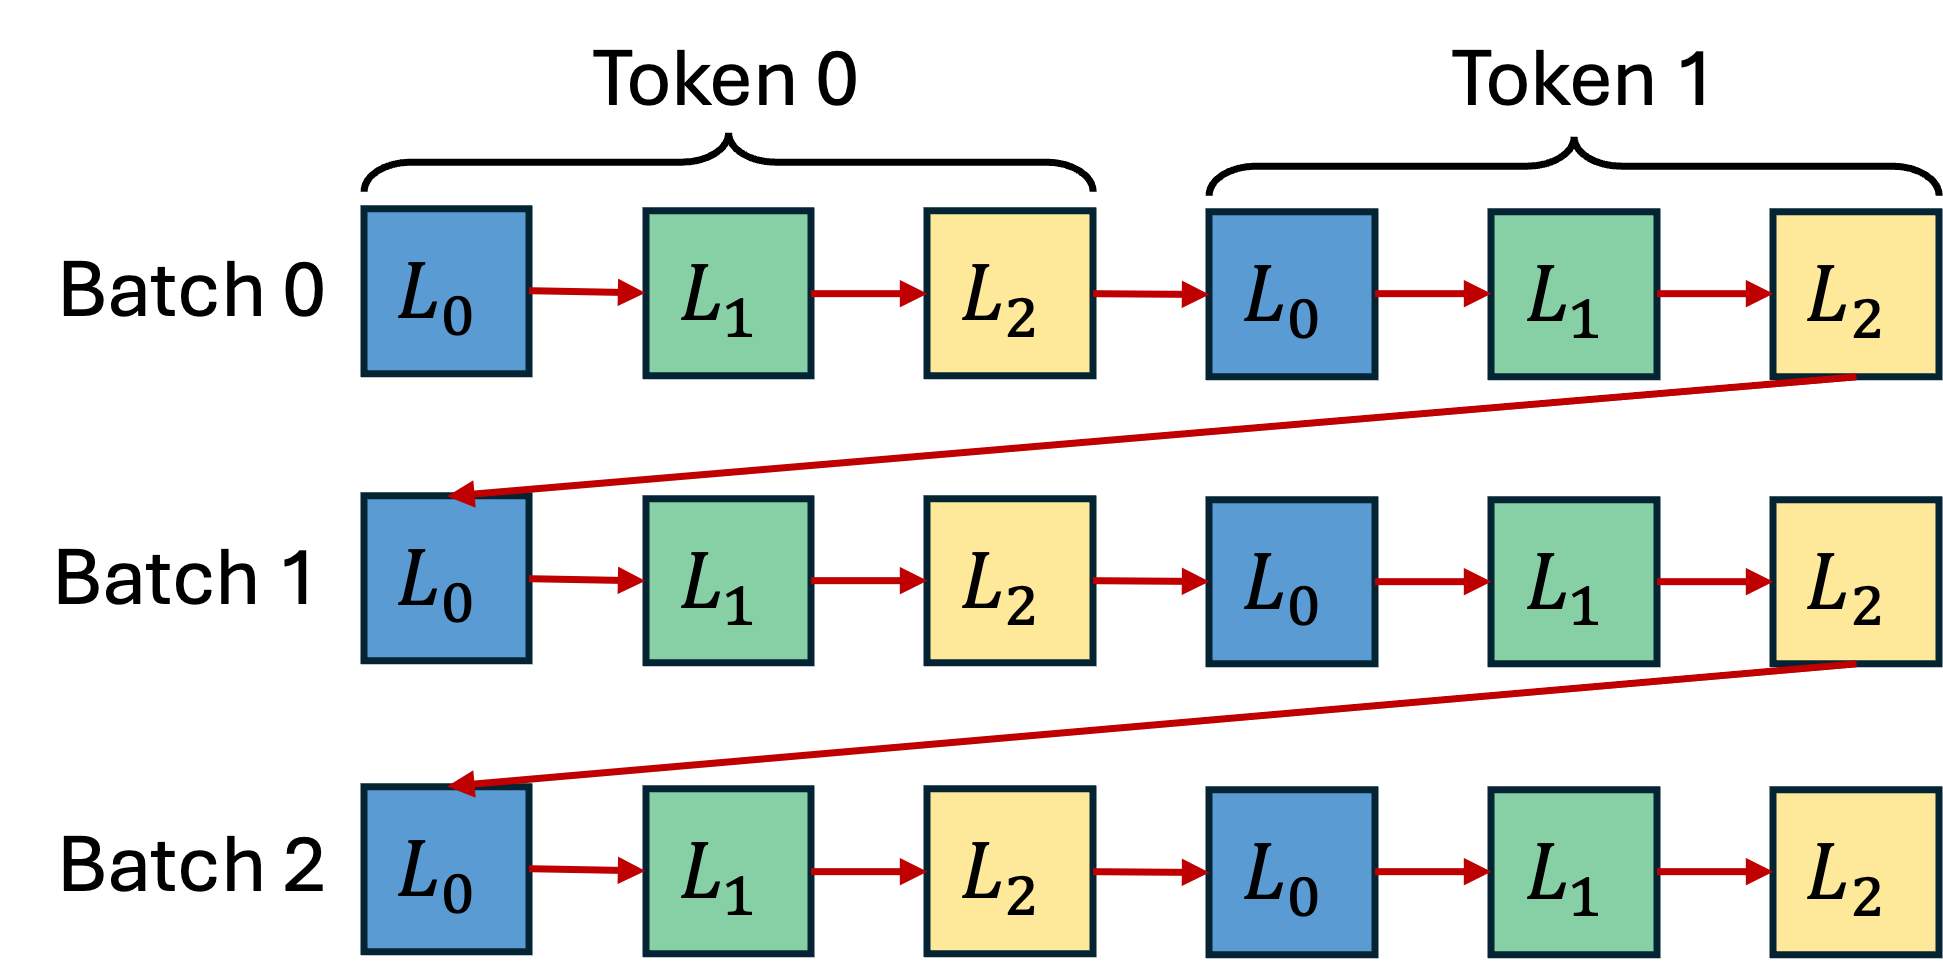
\includegraphics[width=\columnwidth]{assets/11a.png}
\caption{逐行调度。}
\end{subfigure}


\begin{subfigure}[t]{0.9\columnwidth}
\centering
    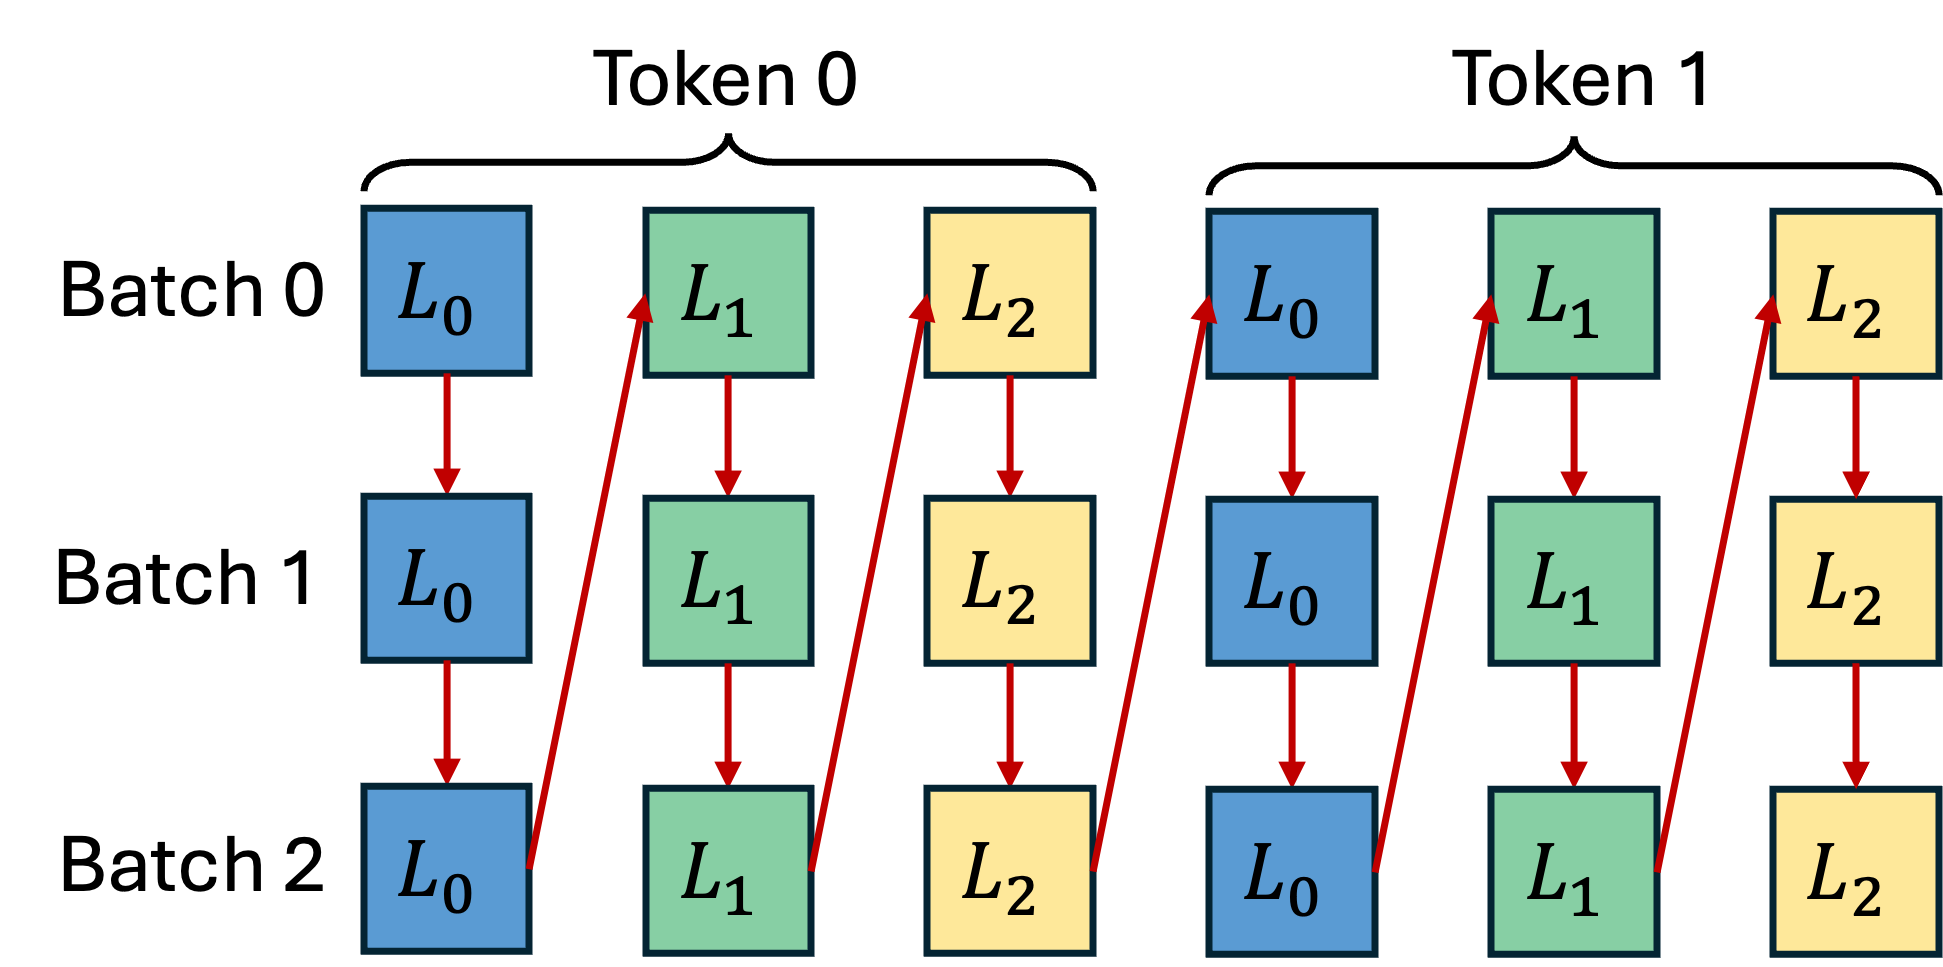
\includegraphics[width=\columnwidth]{assets/11b.png}
\caption{按列调度。}
\end{subfigure}

\caption{两种不同的调度方法，箭头表示调度顺序。}
\label{app:fig:schedule-methods}
\end{figure}



\subsection{带重叠的 KV 缓存部分重计算}
\label{app:overlapping}

基于 FlexGen 构建 \cite{sheng2023flexgen}的计算和通信重叠技术，我们对其进行调整以支持KV 缓存部分重计算。算法 \ref{alg:block_schedule_overlap} 可以同时执行最内层循环中的任务，包括加载下一层的权重、加载 KV 缓存重计算的激活、重计算部分 KV 缓存、加载剩余的 KV 缓存和下一批的激活、存储上一批的 KV 缓存和激活以及执行当前批次的计算。虽然该算法是为逐列调度而设计的，但单批的逐行调度是它的一个特例。


\begin{algorithm}[t!]
\caption{带重叠的 KV 缓存部分重计算}
\label{alg:block_schedule_overlap}
\begin{algorithmic} %[1] enables line numbers
\FOR{$i = 1$ \textbf{to} \texttt{generation\_length}}
    \FOR{$j = 1$ \textbf{to} \texttt{num\_layers}}
        \FOR{$k = 1$ \textbf{to} \texttt{num\_GPU\_batches}}
            \STATE // Load the weight of the next layer
            \STATE \texttt{load\_weight}$(i, j+1, k)$
            
            \STATE // Load the activation for KV cache recomputation of the next batch
            \STATE \texttt{load\_activation\_recompute}$(i, j, k+1)$
            
            \STATE // Load the KV cache and activation of the next batch
            \STATE \texttt{load\_cache}$(i, j, k+1)$
            \STATE \texttt{load\_activation}$(i, j, k+1)$
            
            \STATE // Compute this batch
            \STATE \texttt{compute}$(i, j, k)$
            
            \STATE // Store the KV cache and activation of the previous batch
            \STATE \texttt{store\_activation}$(i, j, k-1)$
            \STATE \texttt{store\_cache}$(i, j, k-1)$
            
            \STATE // Synchronize all devices
            \STATE \texttt{synchronize}$()$
        \ENDFOR
    \ENDFOR
\ENDFOR
\end{algorithmic}
\end{algorithm}


\subsection{详细实验结果}
\label{app:detailed-exp}
表 \ref{app:tab:opt-6.7b} 和 \ref{app:tab:opt-13b} 展示了使用 OPT-6.7B 和 OPT-13B 的面向延迟的工作负载的详细实验结果。结果显示了之间的性能差异 {\paperName} 以及各种配置的 GPU 峰值内存、解码延迟和吞吐量方面的基线（带有 KV 缓存卸载的 Hugging Face Transformer）。尤其， {\paperName} 始终如一地实现较低的延迟，同时保持可比较的内存使用量。


\begin{table*}[h]
\centering
\resizebox{\textwidth}{!}{%
\begin{tabular}{cccccccc}
\hline
\multicolumn{1}{l}{Method} & Batch size & \begin{tabular}[c]{@{}c@{}}Prompt\\ length\end{tabular} & \begin{tabular}[c]{@{}c@{}}Generation \\ length\end{tabular} & \begin{tabular}[c]{@{}c@{}}Cache size \\ (GB)\end{tabular} & \begin{tabular}[c]{@{}c@{}}GPU peak mem \\ (GB)\end{tabular} & \begin{tabular}[c]{@{}c@{}}Decode latency\\ (sec)\end{tabular} & \begin{tabular}[c]{@{}c@{}}Decode throughput\\ (tokens/s)\end{tabular} \\ \hline
\multirow{6}{*}{Accel.} & 64 & 128 & 32 & 5.0 & 14.427 & 8.905 & 222.788 \\ \cline{2-8} 
 & 64 & 128 & 128 & 8.0 & 14.708 & 71.327 & 113.954 \\ \cline{2-8} 
 & 64 & 256 & 32 & 9.0 & 16.337 & 26.825 & 73.961 \\ \cline{2-8} 
 & 64 & 256 & 128 & 12.0 & 16.618 & 88.354 & 91.993 \\ \cline{2-8} 
 & 64 & 512 & 32 & 17.0 & 20.154 & 24.390 & 81.344 \\ \cline{2-8} 
 & 64 & 512 & 128 & 20.0 & 20.576 & 110.277 & 73.705 \\ \hline
\multirow{6}{*}{{\paperName}} & 64 & 128 & 32 & 5.0 & 14.364 & 6.651 & 298.284 \\ \cline{2-8} 
 & 64 & 128 & 128 & 8.0 & 14.645 & 45.766 & 177.598 \\ \cline{2-8} 
 & 64 & 256 & 32 & 9.0 & 16.212 & 19.138 & 103.666 \\ \cline{2-8} 
 & 64 & 256 & 128 & 12.0 & 16.493 & 61.597 & 131.955 \\ \cline{2-8} 
 & 64 & 512 & 32 & 17.0 & 19.904 & 20.349 & 97.501 \\ \cline{2-8} 
 & 64 & 512 & 128 & 20.0 & 20.951 & 93.932 & 86.531 \\ \hline
\end{tabular}
}
\caption{对应图 \ref{fig:latency-exp} 的 OPT-6.7B 详细实验结果。}
\label{app:tab:opt-6.7b}
\end{table*}


\begin{table*}[h]
\centering
\resizebox{\textwidth}{!}{%
\begin{tabular}{cccccccc}
\hline
\multicolumn{1}{l}{Method} & Batch size & \begin{tabular}[c]{@{}c@{}}Prompt\\ length\end{tabular} & \begin{tabular}[c]{@{}c@{}}Generation \\ length\end{tabular} & \begin{tabular}[c]{@{}c@{}}Cache size \\ (GB)\end{tabular} & \begin{tabular}[c]{@{}c@{}}GPU peak mem \\ (GB)\end{tabular} & \begin{tabular}[c]{@{}c@{}}Decode latency\\ (sec)\end{tabular} & \begin{tabular}[c]{@{}c@{}}Decode throughput\\ (tokens/s)\end{tabular} \\ \hline
\multirow{6}{*}{Accel.} & 64 & 128 & 32 & 7.812 & 26.083 & 11.409 & 173.891  \\ \cline{2-8} 
 & 64 & 128 & 128 & 12.500 & 26.434 & 73.896 & 109.993 \\ \cline{2-8} 
 & 64 & 256 & 32 & 14.062 & 28.087 & 19.381 & 102.368 \\ \cline{2-8} 
 & 64 & 256 & 128 & 18.750 & 28.439 & 104.115 & 78.068 \\ \cline{2-8} 
 & 64 & 512 & 32 & 26.562 & 32.851 & 35.066 & 56.579 \\ \cline{2-8} 
 & 64 & 512 & 128 & 31.250 & 34.146 & 168.155 & 48.336 \\ \hline
\multirow{6}{*}{{\paperName}} & 64 & 128 & 32 & 7.812 & 26.005 & 9.148 & 216.867 \\ \cline{2-8} 
 & 64 & 128 & 128 & 12.500 & 26.356 & 66.119 & 122.929 \\ \cline{2-8} 
 & 64 & 256 & 32 & 14.062 & 27.931 & 16.654 & 119.127 \\ \cline{2-8} 
 & 64 & 256 & 128 & 18.750 & 28.337 & 88.492 & 91.850 \\ \cline{2-8} 
 & 64 & 512 & 32 & 26.562 & 33.203 & 29.215 & 67.911 \\ \cline{2-8} 
 & 64 & 512 & 128 & 31.250 & 34.615 & 138.377 & 58.738 \\ \hline
\end{tabular}
}
\caption{对应图 \ref{fig:latency-exp} 的 OPT-13B 详细实验结果。}
\label{app:tab:opt-13b}
\end{table*}

\subsection{最优 KV 缓存切分点}
\label{app:optimal-split-points}

图 \ref{app:fig:split-points} 给出最优的KV 缓存分割点 $l$，通过求解式中定义的线性规划问题得到~\eqref{eq:lp}，用于第 1 节中面向延迟的工作负载实验的第一个设置 \ref{sec:exp} （提示长度为128，生成长度为32）。基于系统分析统计和KV 缓存大小，最佳分割点 $l$ 当生成长度为 1 时，为 182，并且 $l$ 当生成长度为 32 时，增加到 128。


\begin{figure}[h]
\centering
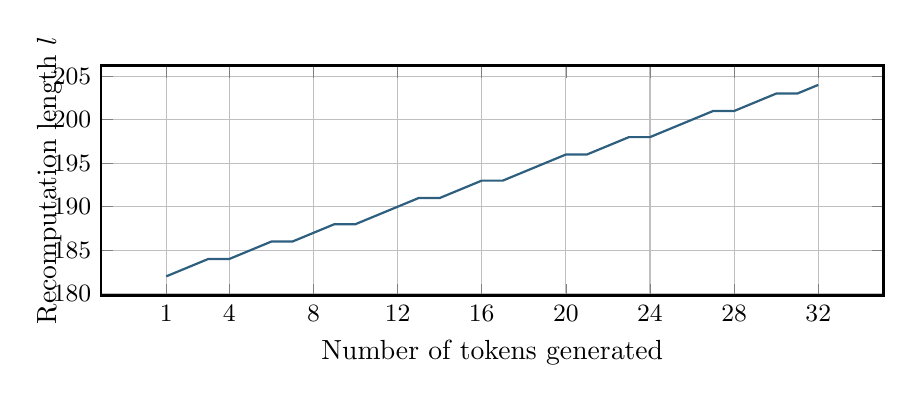
\begin{tikzpicture}
    \begin{axis}[
        axis line style={line width=1pt},
        width=0.95\columnwidth,
        height=4.5cm,
        xlabel={Number of tokens generated},
        ylabel={Recomputation length $l$},
        ylabel style={yshift=-10pt},
        tick label style={font=\small},
        grid=both,
        xtick={1,4,8,12,16,20,24,28,32}, 
        ytick={180,185,190,195,200,205}, 
    ]
    \addplot[color=darkteal, thick] coordinates {
        (1, 182) (2, 183) (3, 184) (4, 184) (5, 185) (6, 186) 
        (7, 186) (8, 187) (9, 188) (10, 188) (11, 189) (12, 190) 
        (13, 191) (14, 191) (15, 192) (16, 193) (17, 193) 
        (18, 194) (19, 195) (20, 196) (21, 196) (22, 197) 
        (23, 198) (24, 198) (25, 199) (26, 200) (27, 201) 
        (28, 201) (29, 202) (30, 203) (31, 203) (32, 204)
    };
    \end{axis}
\end{tikzpicture}
\caption{生成过程中最优 KV 缓存分割点 $l$ 的变化。}
\label{app:fig:split-points}
\end{figure}


\subsection{低端 GPU上的系统性能}
\label{app:low-end-gpu-experiments}

为了进一步证明其适应性 {\paperName}，我们在低端系统上对其进行评估，该系统配备 AMD EPYC 32 核 CPU 和 NVIDIA Quadro RTX 5000 GPU（16 GB HBM，89.2 TFLOPS FP16 峰值性能），通过 PCIe 4.0 x8（16 GB/s 带宽）连接。此系统设置中的 GPU TFLOPS、GPU 内存和 PCIe 带宽低于我们之前使用的默认系统中的值。尽管 GPU 速度和带宽降低了， {\paperName} 达到 15\% 在相同的面向吞吐量的工作负载中，OPT-6.7B 的吞吐量高于 FlexGen，如表所示 \ref{tab:throughput_exp}. 


\begin{table}[h]
\centering
\resizebox{\columnwidth}{!}{%
\begin{tabular}{ccccccc}
\hline
\textbf{Seq len} & \textbf{256/32} & \textbf{256/128} & \textbf{512/32} & \textbf{512/128} & \textbf{1024/32} & \textbf{1024/128} \\ \hline
% \multirow{2}{*}{OPT-6.7B} 
 FlexGen & 50.057 & 46.779 & 29.614 & 28.650 & 15.778 & 16.194 \\ \hline
 {\paperName}    & 53.976 & 49.860 & 33.666 & 32.277 & 18.285 & 18.108 \\ \hline
% \multirow{2}{*}{OPT-13B} 
 % & FlexGen &  &  &  &  &  &  \\ \cline{2-8}
 % & {\paperName}    &  &  &  &  &  &  \\ \hline
\end{tabular}
}
\caption{低端 GPU 系统上的吞吐量（令牌/秒）比较。}
\label{tab:throughput_exp}
\end{table}


\subsection{LLaMa 模型上的补充实验结果}

除了小节讨论的OPT模式之外~\ref{sec:exp}，我们对最新的 LLaMa2-7B 和 LLaMa2-13B 模型进行了进一步的实验。使用相同的实验设置，我们测量了在不同的提示和生成长度下处理单批大小为 64 的解码吞吐量。如图~\ref{fig:llama-exp}, {\paperName} 在两个 LLaMa2 模型上始终实现比基准（DeepSpeed Inference 和 Hugging Face Accelerate）更高的吞吐量。


\begin{figure}[h]
\centering
\begin{subfigure}{\columnwidth}
    \centering
    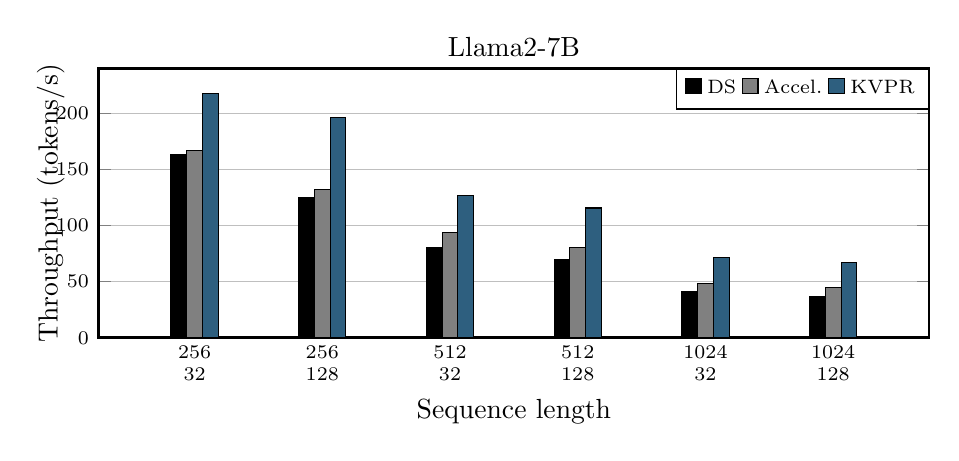
\begin{tikzpicture}
        \begin{axis}[
            axis line style={line width=1pt},
            title={Llama2-7B},
            title style={yshift=-5pt},
            width=\columnwidth,
            height=5cm,
            ybar=0pt,
            bar width=.2cm,
            enlarge x limits=0.15,
            tick label style={font=\scriptsize},
            symbolic x coords={A, B, C, D, E, F},
            xticklabel style={align=center},
            xticklabels={{256 \\ 32}, {256 \\ 128}, {512 \\ 32}, {512 \\ 128}, {1024 \\ 32}, {1024 \\ 128}},
            xtick=data,
            xtick style={draw=none},
            xticklabel style={yshift=5pt, align=center},
            xlabel={Sequence length},
            ylabel={Throughput (tokens/s)},
            ylabel style={yshift=-10pt},
            ymin=0,
            ytick={0, 50, 100, 150, 200, 250},
            grid=major,
            grid style=solid,
            major x grid style={draw=none},
            legend entries={DS, Accel., {\paperName}},
            legend style={at={(1,1)}, anchor=north east, font=\scriptsize, legend cell align=center, legend columns=3},
            legend image code/.code={\draw[yshift=-0.06cm] rectangle (0.2cm,0.2cm);},
        ]

        % DS (7B)
        \addplot[fill=black] coordinates {(A,162.748) (B,124.532) (C,80.215) (D,69.843) (E,40.927) (F,36.482)};

        % HF (7B)
        \addplot[fill=gray] coordinates {(A,166.545) (B,132.054) (C,94.122) (D,80.048) (E,48.599) (F,44.453)};

        % Ours (7B)
        \addplot[fill=darkteal] coordinates {(A,217.822) (B,195.822) (C,126.797) (D,115.597) (E,71.164) (F,66.856)};

        \end{axis}
    \end{tikzpicture}
\end{subfigure}

\begin{subfigure}{\columnwidth}
    \centering
    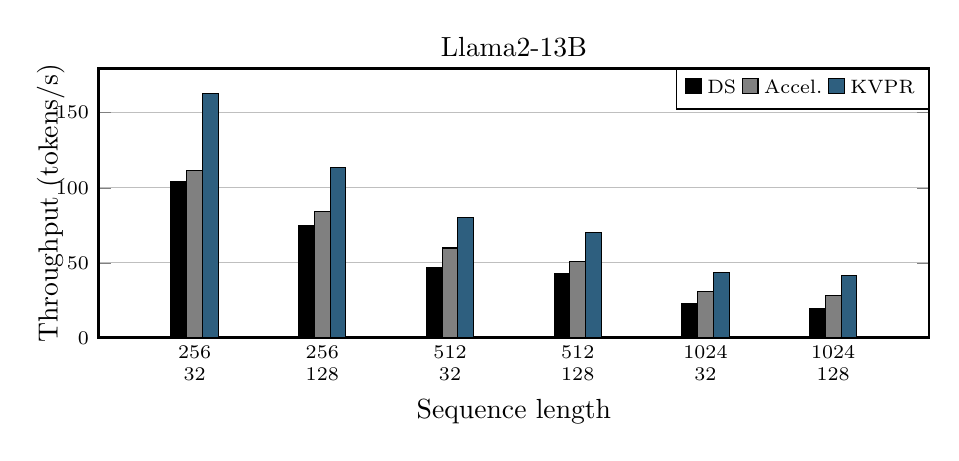
\begin{tikzpicture}
        \begin{axis}[
            axis line style={line width=1pt},
            title={Llama2-13B},
            title style={yshift=-5pt},
            width=\columnwidth,
            height=5cm,
            ybar=0pt,
            bar width=.2cm,
            enlarge x limits=0.15,
            tick label style={font=\scriptsize},
            symbolic x coords={A, B, C, D, E, F},
            xticklabel style={align=center},
            xticklabels={{256 \\ 32}, {256 \\ 128}, {512 \\ 32}, {512 \\ 128}, {1024 \\ 32}, {1024 \\ 128}},
            xtick=data,
            xtick style={draw=none},
            xticklabel style={yshift=5pt, align=center},
            xlabel={Sequence length},
            ylabel={Throughput (tokens/s)},
            ylabel style={yshift=-10pt},
            ymin=0,
            ytick={0, 50, 100, 150, 200},
            grid=major,
            grid style=solid,
            major x grid style={draw=none},
            legend entries={DS, Accel., {\paperName}},
            legend style={at={(1,1)}, anchor=north east, font=\scriptsize, legend cell align=center, legend columns=3},
            legend image code/.code={\draw[yshift=-0.06cm] rectangle (0.2cm,0.2cm);},
        ]

        % DS (13B)
        \addplot[fill=black] coordinates {(A,104.382) (B,75.129) (C,46.735) (D,42.647) (E,22.914) (F,19.526)};

        % HF (13B)
        \addplot[fill=gray] coordinates {(A,111.248) (B,84.130) (C,59.900) (D,50.966) (E,30.911) (F,28.360)};

        % Ours (13B)
        \addplot[fill=darkteal] coordinates {(A,163.078) (B,113.390) (C,80.158) (D,70.169) (E,43.429) (F,41.284)};

        \end{axis}
    \end{tikzpicture}
\end{subfigure}

\caption{跨不同序列长度的单个批量大小为 64 的解码吞吐量。}
\label{fig:llama-exp}
\end{figure}



\subsection{分布式系统设置与CPU辅助方法的比较}
\label{app:comparing-cpu}

在本实验中，我们比较了 CPU 辅助卸载方法 FastDecode 的性能 \cite{he2024fastdecode}， 和 {\paperName} 在配备 8 个 NVIDIA A100 GPU 和一个 CPU 的 GPU 节点上，这是相同的 AMD EPYC 处理器（64 核，PCIe 4.0 128 通道），如第 1 节中所述 \ref{sec:exp}。

我们运行 FastDecode 的多个并发进程 {\paperName} 在可用的 GPU 上，每个 GPU 专用于一个进程。此设置模拟多个用户共享单个计算节点或单个用户执行数据并行推理的场景。 FastDecode 依赖 CPU 进行注意力计算，当管理多个并发推理进程时，CPU 成为瓶颈，导致性能下降。相比之下， {\paperName} 完全消除了对 CPU 的依赖，并优化了 PCIe 总线上的数据传输。 

图 \ref{app:fig:cpu} 表明虽然 FastDecode 的吞吐量随着进程数量的增加而显著下降， {\paperName} 表现出更好的可扩展性，在单CPU和多 GPU的系统中保持稳定的性能。

\begin{figure}[h]
\centering
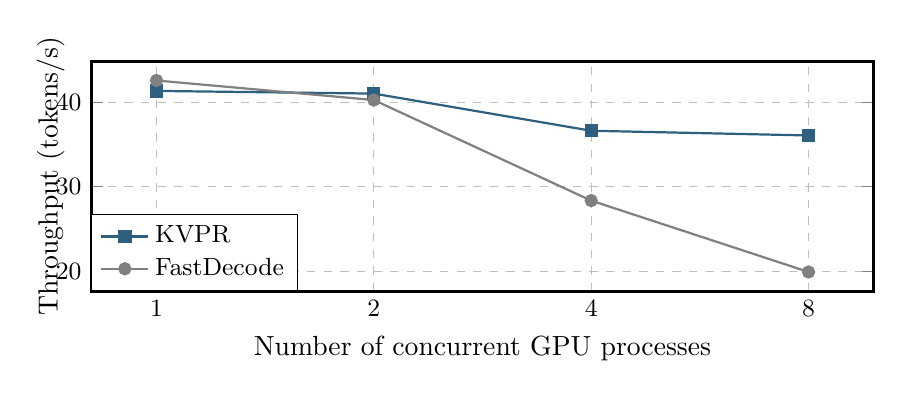
\begin{tikzpicture}
    \begin{axis}[
        axis line style={line width=1pt},
        width=0.95\columnwidth,
        height=4.5cm,
        xlabel={Number of concurrent GPU processes},
        ylabel={Throughput (tokens/s)},
        ylabel style={yshift=-10pt},
        xtick={1,2,3,4},
        xticklabels={1,2,4,8},
        xtick style={draw=none},
        grid=both,
        major grid style={dashed},
        minor grid style={dotted},
        tick label style={font=\small},
        legend entries={{\paperName}, FastDecode},
        legend style={at={(0,0)}, anchor=south west, font=\small, row sep=0cm, column sep=0cm, legend cell align=left},
    ]
    \addplot[color=darkteal, mark=square*, thick] coordinates {
        (1, 41.343)
        (2, 41.026)
        (3, 36.626)
        (4, 36.069)
    };    
    \addplot[color=gray, mark=*, thick] coordinates {
        (1, 42.579)
        (2, 40.263)
        (3, 28.354)
        (4, 19.903)
    };
    \end{axis}
\end{tikzpicture}
\caption{{\paperName} 与 FastDecode 在不同 GPU 工作负载下的吞吐量比较。}
\label{app:fig:cpu}
\end{figure}



\subsection{扩展相关工作}
\textbf{GPU 高效的 LLM 推理。} 
最大化 GPU 利用率对于高效服务LLM以实现低延迟和高吞吐量至关重要。
Orca \cite{yu2022orca} 采用迭代级调度来处理具有不同输出长度的批次，立即返回完成的序列以服务新的序列。 
% \textcolor{red}{S3 \cite{}} builds upon this approach by predicting output sequence lengths in advance to optimize resource allocation. 
PagedAttention \cite{kwon2023vllm} 观察到 KV 缓存会随 token 生成动态增长和收缩，且序列生命周期和长度并不能预先确定。它通过将 KV 缓存管理为非连续内存块来解决这一问题。FlashAttention \cite{dao2022flashattention} 将注意力操作融合到单个内核中，并将 QKV 矩阵分割为更小块，以优化 GPU SRAM 使用并减少 HBM 访问开销，而我们的工作主要关注 PCIe 带宽优化。DeepSpeed Inference \cite{aminabadi2022deepspeed} 结合 GPU 内存以及 CPU/NVMe 混合推理技术，增强了密集和稀疏 Transformer 模型的多 GPU 推理。Flash Decoding \cite{flashdecoding2023} 通过将键和值切分为更小块，实现并行注意力计算并组合最终输出，加速长上下文推理。HCache \cite{gao2025fast} 关注在在线推理中跨用户请求恢复并复用上下文状态，在延迟、容量和持久性之间取得平衡，以实现稳健的 LLM 服务。

\noindent \textbf{KV 缓存优化。} 
高效的 KV 缓存管理通过压缩或驱逐策略增强推理性能。KIVI \cite{liu2024kivi} 引入了免调整 2 位量化方法来压缩每个通道的键缓存和每个令牌的值缓存。同样，KVQuant \cite{hooper2024kvquant} 通过将每通道量化与 LLaMA 的预旋转位置嵌入量化相结合，应用 3 位压缩。对于驱逐，H2O \cite{zhang2023h2o} 将 KV 缓存驱逐制定为动态子模块问题，优先考虑关键和最近的令牌以提高吞吐量。StreamingLLM \cite{xiao2023efficient} 使用窗口注意力和固定大小的滑动窗口来保留最新的 KV 缓存，一旦缓存达到容量，就保持恒定的内存使用和解码速度。InfiniGen \cite{lee2024infinigen} 将低等级键缓存存储在 GPU 内存中，将值缓存卸载到 CPU，并根据近似注意力分数选择性地检索重要值。

\end{document}
